\documentclass{article}

\usepackage{geometry}
\geometry{a4paper,scale=0.8,centering}

\usepackage[UTF8,heading=true]{ctex}

\usepackage{times}
\usepackage{caption}
\usepackage{subcaption}
\usepackage{latexsym}
\usepackage{tikz}
\usepackage{hyperref}
\usepackage{comment}
\usetikzlibrary{arrows}
\usetikzlibrary{positioning,shadows.blur}

\renewcommand{\labelitemi}{\ding{112}}
\usepackage{amsmath}
\usepackage{amssymb}
\usepackage{xifthen}

\usepackage{graphicx}
\usepackage{graphics}
\graphicspath{ {./figures/} }

\usepackage{booktabs}
\usepackage{makecell}
\usepackage{array}

\usepackage{float}
\usepackage{algorithm}
\usepackage[noend]{algpseudocode}

\DeclareMathOperator*{\argmax}{\arg\!\max}
\usetikzlibrary{shapes.geometric, arrows, patterns, decorations.pathreplacing}

\newcommand{\them}[0]{\textbf{read:}\ }
\newcommand{\you}[0]{\textbf{write:}\ }


\newcommand{\likelihood}[0]{\textsc{likelihood}\ }
\newcommand{\reinforce}[0]{\textsc{rl}\ }
\newcommand{\rollouts}[0]{\textsc{rollouts}\ }
\newcommand{\rlrollouts}[0]{\textsc{rl+rollouts}\ }

\renewcommand{\vec}[1]{#1}
% 修改脚注
\usepackage{pifont}
\renewcommand{\thefootnote}{\ding{\numexpr171+\value{footnote}}}
\newcommand\wordnote[1]{\footnote{\zihao{5}{#1}}}

\newcommand\quotes[1]{``{#1}''}

\usepackage[super,square,sort]{natbib}

\usepackage{enumitem}

\newcommand{\bmx}[0]{\begin{bmatrix}}
\newcommand{\emx}[0]{\end{bmatrix}}
\newcommand{\qt}[1]{\left<#1\right>}
\newcommand{\qexp}[1]{\left<#1\right>}
\newcommand{\qlay}[1]{\left[#1\right]}
\newcommand{\vect}[1]{\mathbf{#1}}
\newcommand{\vects}[1]{\boldsymbol{#1}}
\newcommand{\matr}[1]{\mathbf{#1}}
\newcommand{\var}[0]{\operatorname{Var}}
\newcommand{\cov}[0]{\operatorname{Cov}}
\newcommand{\diag}[0]{\operatorname{diag}}
\newcommand{\matrs}[1]{\boldsymbol{#1}}
\newcommand{\vone}[0]{\vect{1}}
\newcommand{\va}[0]{\vect{a}}
\newcommand{\vb}[0]{\vect{b}}
\newcommand{\vc}[0]{\vect{c}}
\newcommand{\vh}[0]{\vect{h}}
\newcommand{\vv}[0]{\vect{v}}
\newcommand{\vx}[0]{\vect{x}}
\newcommand{\vw}[0]{\vect{w}}
\newcommand{\vs}[0]{\vect{s}}
\newcommand{\vf}[0]{\vect{f}}
\newcommand{\ve}[0]{\vect{e}}
\newcommand{\vy}[0]{\vect{y}}
\newcommand{\vg}[0]{\vect{g}}
\newcommand{\vr}[0]{\vect{r}}
\newcommand{\vm}[0]{\vect{m}}
\newcommand{\vu}[0]{\vect{u}}
\newcommand{\vL}[0]{\vect{L}}
\newcommand{\vz}[0]{\vect{z}}
\newcommand{\vp}[0]{\vect{p}}
\newcommand{\mO}[0]{\matr{O}}
\newcommand{\mC}[0]{\matr{C}}
\newcommand{\mW}[0]{\matr{W}}
\newcommand{\mG}[0]{\matr{G}}
\newcommand{\mX}[0]{\matr{X}}
\newcommand{\mQ}[0]{\matr{Q}}
\newcommand{\mU}[0]{\matr{U}}
\newcommand{\mV}[0]{\matr{V}}
\newcommand{\mL}[0]{\matr{L}}
\newcommand{\mR}[0]{\matr{R}}
\newcommand{\mA}{\matr{A}}
\newcommand{\mD}{\matr{D}}
\newcommand{\mS}{\matr{S}}
\newcommand{\mI}{\matr{I}}
\newcommand{\td}[0]{\text{d}}
\newcommand{\vsig}[0]{\vects{\sigma}}
\newcommand{\valpha}[0]{\vects{\alpha}}
\newcommand{\vmu}[0]{\vects{\mu}}
\newcommand{\tf}[0]{\text{m}}
\newcommand{\tdf}[0]{\text{dm}}
\newcommand{\TT}[0]{{\vects{\theta}}}
\newcommand{\grad}[0]{\nabla}
\newcommand{\alert}[1]{\textcolor{red}{#1}}
\newcommand{\N}[0]{\mathcal{N}}
\newcommand{\LL}[0]{\mathcal{L}}
\newcommand{\HH}[0]{\mathcal{H}}
\newcommand{\RR}[0]{\mathbb{R}}
\newcommand{\Scal}[0]{\mathcal{S}}
\newcommand{\sigmoid}{\sigma}
\newcommand{\softmax}{\text{softmax}}
\newcommand{\E}[0]{\mathbb{E}}
\newcommand{\enabla}[0]{\ensuremath{%
    \overset{\raisebox{-0.3ex}[0.5ex][0ex]{%
    \ensuremath{\scriptscriptstyle e}}}{\nabla}}}
\newcommand{\enhnabla}[0]{\nabla_{\hspace{-0.5mm}e}\,}
\newcommand{\tred}[1]{\textcolor{red}{#1}}

\DeclareMathOperator*{\argmin}{arg\,min}
% \DeclareMathOperator*{\argmax}{arg\,max}

\title{\heiti{}\zihao{3} 在线呼叫中心的智能客服问答机器人
}
\author{张心泽}
\date{\today}

\begin{document}
    
    \maketitle

    \section*{前言}
\zihao{-4}
\label{section:before}

呼叫中心(Call Center)又称为客户服务中心,是基于CTI技术\wordnote{
    CTI技术传统的定义为“计算机电话集成”,即Computer Telephony Integration。
    随着电信通信技术的发展,现在的定义为“计算机电信集成”,即Computer Telecommunication Integration。
},利用互联网、电信通信网络和计算机网络的多像功能集成,并与企业连为一体的完整的综合信息服务系统。
早期的呼叫中心依赖电话机或排队机,实现客户电话的纯人工接听。
随着计算机技术、通信技术和电子商务模式的发展,呼叫中心呈现多媒体化、分布式的发展趋势。
现今的呼叫中心架构于IP协议与计算机网络之上,将之前的电话呼叫转变为包括邮件、电话和基于Web2.0技术的在线文本交谈等多种形式,
成为包含通信、计算、管理和业务支撑特性的全媒体交互中心(\citet{马晓军-1})。

然而,新的技术和商业模式在给企业创造利润、引领企业进行销售与服务模式变革的同时,也给企业带来了新的挑战。
以阿里巴巴淘系为例,包含淘宝、咸鱼等在内的电商平台具有亿量级的在线商品库,用户数同样在数亿规模。
每天淘系平台会产生包含购物、物流和售后咨询在内的海量服务请求。
即便具有现代的呼叫中心,简单但繁复的问题咨询仍给企业带来了庞大的人工成本。

因此本文从呼叫中心的核心功能即客服问答出发,结合机器学习等人工智能技术、方法、模型和算法,
分析和设计一种智能客服问答机器人(以下简称智能客服),以帮助企业降低人工客服工作量和提高服务资源使用效率。

在此本文题目要求为:“呼叫中心的AI接线员的系统的设计与实现”,并有以下三点具体要求:

\begin{enumerate}[leftmargin=3.5em,itemindent=0em,label=(\arabic*),itemsep=0pt,topsep=0pt]
    \item[\textasteriskcentered] 呼叫中心的AI接线员的系统的设计与实现
    \item 
    调研目前国内外最好的三家(款)系统。对比它们的功能、性能和可用性等相关指标,指出它们的优缺点;
    \item 
    完成总结报告和汇报PPT,解释其主要工作原理和实现方式(如何训练模型和算法、如何实现应用),附演示视频;
    \item 
    提出具体研究和实施方案,
    即如何用机器学习等人工智能的技术、方法、模型和算法来实现面向特定领域的对话机器人
    (如替代电信114接线员)。
\end{enumerate}

基于时间因素和论文篇幅,本文结合实际情况对要求进行了适当松弛,并对相关概念进行了界定。

基于Web2.0技术的在线文本交谈已成为呼叫中心客服与用户交互的主要形式。
虽然电话和邮件等形式通过语音识别、分句等处理也可转化为文本交谈,
但其属于另外相对独立的研究领域,不在本文研究范畴。
因此本文并不考虑呼叫中心的电话、邮件等交互形式,
而以在线文本交谈为情景,设计和实现智能客服问答机器人即“AI接线员”。

呼叫中心的智能客服目前尚处发展阶段,缺乏统一和公认的评价体系。
因此本文无法界定“最好”,在此通过经验确定了相关评价指标,挑选和对比了国内外三家具有代表性的此类系统。

由于市面上具有代表性的智能客服系统尚未开源,因此无法准确得知其原理细节和实现方式。
在此,本文通过官网展示或演示视频,结合现有研究,对其工作原理和实现方式进行合理推测。

综上所述,本文以呼叫中心在线文本交谈为情景,
调研了国内外三家具有代表性的客服智能问答系统,建立了相关评价指标进行对比,
推断了其主要工作原理和实现方式,并具体提出了一种面向客服领域的智能问答机器人。

    \section{介绍}
\zihao{-4}
\label{section:introduction}

% 对话机器人作为现在和未来各种服务的入口,是当前人工智能领域的热门研究方向。

% 国内外已出现了诸多类型的对话机器人,
% 以应用目的(以“\textbullet”标识)和技术手段(以“\dag”标识)进行划分,
% 可有以下两种分类方法。

% \begin{enumerate}[leftmargin=3.5em,itemindent=0em,label=(\arabic*),itemsep=0pt,topsep=0pt]
%     \item[\textbullet] 
%     目标驱动(Goal-based):目标驱动对话机器人具有明确的服务目标、对象或用途,
%     如Facebook Negotiation谈判机器人、阿里Alime客服机器人、Disrupt 911bot报警机器人等,
%     是面向特定用途的对话机器人;
%     \item[\textbullet]
%     无目标驱动(Non Goal-based):
%     与目标驱动机器人不同,
%     以微软Cortana、苹果Siri、谷歌Assitant为代表的无目标驱动对话机器人指代
%     并非面向特定领域或服务目的,提供搜索资料、进行终端设置、调用终端功能和聊天等各种服务的对话机器人。
%     这种对话机器人没有明确任务目标,也可被称为开放领域的对话机器人。
%     \item[\dag]
%     检索式:检索式对话机器人指事先具有知识库,对话系统接受到用户的输入句子后,
%     通过在知识库中以搜索匹配的方式进行应答内容提取;
%     \item[\dag]
%     提出具体研究和实施方案,
%     即如何用机器学习等人工智能的技术、方法、模型和算法来实现面向特定领域的对话机器人
%     (如替代电信114接线员)。
% \end{enumerate}

% 目标驱动(Goal-based):目标驱动对话机器人具有明确的服务目标、对象或用途,
% 如Facebook Negotiation谈判机器人、阿里Alime客服机器人、Disrupt 911bot报警机器人等,
% 是面向特定用途的对话机器人;

% 无目标驱动(Non Goal-based):
% 与目标驱动机器人不同,
% 以微软Cortana、苹果Siri、谷歌Assitant为代表的无目标驱动对话机器人指代
% 并非面向特定领域或服务目的,提供搜索资料、进行终端设置、调用终端功能和聊天等各种服务的对话机器人。
% 这种对话机器人没有明确任务目标,也可被称为开放领域的对话机器人。

从早起的图书情报检索系统、电信114服务系统到现在的在线呼叫中心,
快速并准确的获取与反馈信息一直是用户和企业的追求目标。
% 尤其是在信息呈现规模巨大、模态多样、关联复杂和真假难辨的大数据时代。
% 一方面,用户的需求愈加多样,基于关键词抽取的主题相关模型或或基于浅层语义分析的检索系统已不能满足用户的需求;
% 另一方便,企业的服务更加精细,希望提供更加类人的自然语言应答,以减轻人工客服的压力,优化企业的服务资源配置。
伴随而生的智能问答系统已有近70年的发展历史。
早期的智能问答系统大多数针对特定问题设计,
且由于技术和环境的限制数据量十分有限,不易进行扩展和训练,如\citet{Green-2}和\citet{Woods-3}。
这些诞生在上世界六七十年代的智能问答系统仅接受特定形式的自然语言语句,且供系统训练的数据也很少,
无法进行较广范围的问答从而未被广泛使用。

进入九十年代后,借助互联网技术的发展,大量可供训练的问答对在网上可被搜索和爬取,进而构建特定主题下的语料库
\citep{dang2007overview}。
这些语料库的出现极大促进了智能问答系统的发展,研究人员在这些语料库上训练和测试各种问答模型,
先后提出了基于逻辑推理\citep{moldovan2001logic}、
基于模式匹配\citep{soubbotin2001patterns}和
基于机器学习\citep{yang2002integration}等许多方法。
在此阶段,人们主要利用信息检索或浅层语义理解去候选应答集中寻找应答从而构建智能问答系统,
故将此类系统归纳为检索式问答系统。但检索式问答存在固有缺陷。应答的准确与否很大程度上取决于当前问句的信息充分程度,
一方面,不能很好的关联该问句的上下;另一方面,问答系统的训练依赖当前问句抽取后表述的标签或是关联规则。
因此检索式问答系统对短问句的应答效果欠佳,且规则构建仍需要较高的人力或专家知识。

随着深度学习方法在学界和业界均取得了较好的效果,研究人员将端到端的思想应用在了智能问答系统,面向不同特定领域提出了
基于端到端的统计机器翻译\citep{cho2014learning}、
机器阅读理解\citep{tan2017s}和机器谈判代理\citep{lewis2017s}等许多模型。
在此阶段,人们利用词嵌入(Word Embedding)、编-解码(Encode-Decode)和
改进型循环神经网络(如LSTM、GRUs)等方法生成应答文本,
故将此类系统归纳为生成式问答系统。
虽然生成式系统能够一定程度地解决长问句和问句的上下文理解难题,
但生成式问答同样存在弊端。
一方面,相较于基于规则或搜索的检索式系统,在处理已存在语义库和知识库的问答对时,
可能需要上千次对话训练才能达到检索式问答系统几次简单设置(构建规则)的效果;
另一方面,虽然生成式系统能够记忆上文甚至推演下文\citep{lewis2017s}给用户一种在和人类对话的感觉,
然而,这种模型很难训练,在进行长应答时很可能会犯语法错误。
因此生成式系统相对检索式系统需要更多的对话训练数据。

目前,基于检索式或生成式的问答系统都可应用于对话机器人,但在面对开放领域和特定领域时,两者各有优劣。
在面对开放领域时,典型如较纯粹聊天场景,
此时用户的话题并不面向特定领域和具有特定目的或任务,希望得到类人的自然语言问答体验,
因此生成式问答模型在面向开放领域即无任务驱动下具有天然的优势,
此类对话机器人有微软“小冰”、Facebook“Messenger”和Github“Hubot”等。
而在面对特定领域,典型如呼叫中心,用户与对话机器人均面向特定领域和具有特定目的或任务,
此时用户更希望对话机器人能够准确回答领域内问题。
因此检索式问答模型在面向特定领域即任务驱动下更具有优势,
此类对话机器人如面向报警的Disrupt“911bot”\citep{911bot}、
面向在线客服的阿里“ALIME”\citep{alimi}、京东“JIMI”\citep{jimi}和网易“七鱼”\citep{wangyiqiyu}等。

近年来,
基于WordNet、HowNet等词汇知识库和Wikipedia与电商数据这种动态更新的知识资源库,
大规模知识图谱日益成熟;
同时,基于统计机器学习的自然语言处理和基于深度学习的知识推理技术有了快速发展
;此外,CUDA加速计算的出现大大降低了机器学习与深度学习带来的庞大计算开销。
这三方面的进步分别为智能问答系统的发展奠定了资源、技术和成本基础,
给智能问答系统的发展带来了新的契机。

值得关注的是,随着深度学习的浪潮,使用深度学习完成任务驱动下的问答模型成为具有技术优势的学界主流;
而在具有资源优势的业界,以智能客服为代表的任务驱动问答模型却几乎都采用更实用的检索式问答模型。
如何通过深度学习对接包含词典、规则和知识图谱在内的知识,使检索式问答模型与生成式问答模型巧妙融合,
达到学界和业界优势互补,是当前厄待解决的问题。

本文基于在线呼叫中心面向客服领域,首先对比国内外具有代表性的呼叫中心智能客服系统,
合理推测其工作原理和实现方式,并进行对比与评价;
随后融合统计机器学习与知识,总结了一套“生成-检索-生成”流程,
提出一种混合式的端到端智能问答系统。

    \section{业界智能客服系统现状}
\zihao{-4}
\label{section:peer-system}

本文基于在线呼叫中心面向客服领域,选择了当前具有代表性的三家(款)呼叫中心智能客服系统,
阿里“ALIME”、京东“JIMI”和网易“七鱼”进行分析、对比和评价。
由于包括这三家在内的业内主要智能客服问答系统均为开源,因此本文根据其网站介绍、演示Demo和使用说明
对其工作原理和实现方式进行合理推测,并建立一套评价标准,对其进行对比和评价。

\subsection{ALIME}
\label{subsection:alime}
阿里“ALIME”是阿里巴巴推出的在线呼叫中心客服对话机器人平台,其核心场景为:
在商家促销活动时(如“年中6·18”、“双11”等)人工客服资源紧张,无法顾及到所有顾客,
此时,若顾客无法及时得到关于商品信息的应答,则销售机会转瞬即逝,给商家带来损失;
在平常时段,大型商家具有固定的工作时间,往往面临夜间无人或缺人值班的情况,
而小商家则一般身兼数职,分身乏术。因此阿里针对此类场景提出了检索式“ALIME”客服对话机器人平台。

“ALIME”平台系统由“千牛店小蜜”和“阿里小蜜”两部分组成,完整商业版于2017年6月正式上线。
其中“千牛店小蜜”面向淘宝商家,支持所有淘宝和天猫店铺,是阿里商家版智能客服机器人;
“阿里小蜜”面向淘宝顾客,支持所有淘宝顾客,是阿里顾客版智能客服机器人。

“ALIME-千牛店小蜜”(以下简称“店小蜜”)目前主要的功能有:
识别顾客购物意图、判断顾客购物缺失信息、查询顾客购物信息和一定时限内上下文识别等。
具体产品功能和知识库见表\ref{table:alime-ability}和表\ref{table:alime-kd}\wordnote{
    其中,“—”表示无,“...”表示省略。
}
。
\begin{table*}[h]

\parbox[t]{0.5\textwidth}{
\centering
\caption{\label{table:alime-ability} “ALIME-千牛店小蜜”产品能力}

\begin{tabular}{ccc}
\toprule
售前服务  &   订单服务  &   售后服务\\
\midrule
回复询价    &   回复发货时间  &   回复退货流程\\
回复询单    &   确认发货快递  &   回复退货事项\\
关联商品回复  &   确认订单修改  &   —\\
解决包邮议价  &   —  &   —\\
回复商品优惠  &   —  &   —\\
回复活动内容  &   —  &   —\\
\bottomrule
\end{tabular}
}
\parbox[t]{0.5\textwidth}{
\centering
\caption{\label{table:alime-kd} “ALIME-千牛店小蜜”电商知识库}

\begin{tabular}{cc}
\toprule
通用知识点 &   行业知识点\\
\midrule
基础商品问题    &   手机行业\\
活动优惠问题    &   服务行业\\
下单付款问题    &   鞋类行业\\
商品物流问题    &   零食行业\\
售后退款问题    &   ...\\
店铺服务问题    &   ...\\
聊天互动问题    &   ...\\
\bottomrule
\end{tabular}
}

\end{table*}

本小节以图\ref{figure:alime_case}为例详细阐述“ALIME”对话过程。
图\ref{figure:alime_case}中展示了“ALIME”的两个对话案例。
其中,图\ref{figure:alime_case1}中为“店小蜜”在服装类淘宝商家“森马”中的应用,即“森小蜜”。
由图可知,顾客:“这件衣服身高160选多大码合适”\wordnote{
    结合后文,这里的“衣服”应该在之前对话中进行过明确。
},
“森小蜜”:“请问体重是多少公斤?”,
顾客:“50”,“森小蜜”:“身高160.0公分,体重50.0公斤,...,推荐[修身M,宽松L]码...”;
图\ref{figure:alime_case2}为“阿里小蜜”在顾客查询中的应用。
\begin{figure*}[ht]
    \centering
    \begin{minipage}{0.5\textwidth}
        \centering
        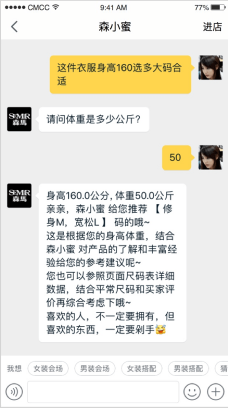
\includegraphics[width=0.6\textwidth]{alime_case1.png}
        \subcaption{\label{figure:alime_case1} “千牛店小蜜”案例}
    \end{minipage}%
    \begin{minipage}{0.5\textwidth}
        \centering
        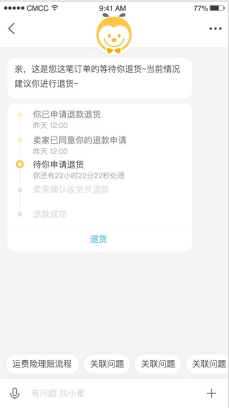
\includegraphics[width=0.6\textwidth]{alime_case2.png}
        \subcaption{\label{figure:alime_case2} “阿里小蜜”案例}
    \end{minipage}%
    \caption{\label{figure:alime_case} 阿里“ALIME”案例}
\end{figure*}

\textbullet{}问答系统首先接收到顾客的输入“这件衣服身高160选多大码合适”。

执行步骤\ding{172}:结合上下文根据语义分析模型对该语句进行分词和关键词抽取。

从该句中抽取关键词“衣服”、“身高”-“160”、“多大”、“码”。
其中,根据“多大”判定该语句为疑问句;
根据“衣服”和上文关联,确定该语句中“衣服”的目标;
根据“键-值”关系“身高-160”和“码”,确定“衣服”的部分商品信息。
综合上述抽取和分析过程,确定该顾客的意图,
即:连接该商家电商服装知识库,查询在“衣服”等于当前衣服、“身高”等于160时的码数,
完成识别购物意图功能。

执行步骤\ding{173}:执行顾客意图,进行检索操作。

此时,根据电商知识库的返回为“衣服”、“身高”、“体重”和“码数”的组合,返回值不唯一,
体现在“码数”和“体重”的返回数量上,因此判定缺失“体重”信息。

执行步骤\ding{174}:询问顾客购物缺失信息。

向顾客提问“体重”信息,以补全购物信息,以获取缺失查询条件“体重”。

\textbullet{}问答系统抛出应答“请问体重是多少公斤”。

\textbullet{}问答系统接受顾客输入“50”。

执行步骤\ding{172}:结合上下文根据语义分析模型对该语句进行分词和关键词抽取。

获取到体重信息“键-值”关系“\mbox{体重}:\mbox{公斤}-50”\wordnote{
    “键-值”关系$pair\{key-value\}$实际是$pair\{index-value\}$关系,即索引-值关系。
    因此键值有多种形式,如上文中身高信息的“键-值”关系为“身高-160”,
    此处体重信息的“键-值”关系为“\mbox{体重}:\mbox{公斤}-50”等。
}
,得到完整顾客信息查询条件。

执行步骤\ding{173}:执行顾客意图,进行检索操作。

此时,根据电商知识库的返回为“衣服”、“身高”、“体重”和“码数”的组合,返回值唯一,获得“码数”信息。

执行步骤\ding{175}:返回顾客购物缺失信息。

\textbullet{}问答系统抛出应答“身高160.0公分,体重50.0公斤,...,推荐[修身M,宽松L]码...”。

这里的问答系统应带内容中虽然带有“推荐”字样,
但实质将查询结果[修身M,宽松L]带入到应答模版“身高*公分,体重*公斤,...,推荐[*]码...”,
并非推荐系统的推荐结果。

\begin{figure*}[!htp]
    \centering
    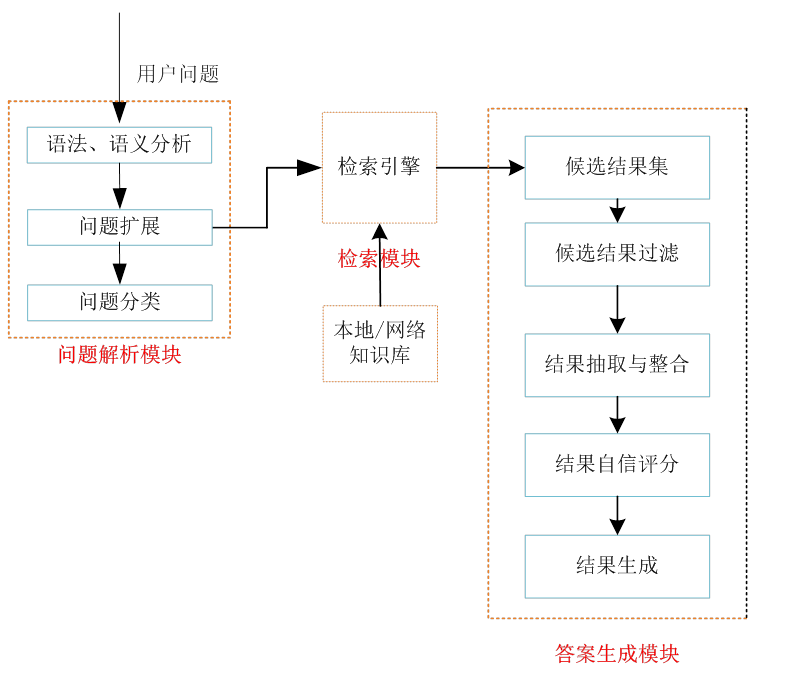
\includegraphics[width=0.8\textwidth]{QA_step.png}
    \caption{\label{figure:qa} 问答系统流程}
\end{figure*}

现阶段业界普遍采用的问答系统流程见图\ref{figure:qa}。

\subsection{JIMI}
\label{subsection:jimi}
京东“JIMI”(JD Instant Messaging intelligence)是京东推出的检索式智能客服机器人,
旨在为京东顾客提供更好的购物和咨询体验。
其应用场景与阿里“ALIME”相同,但比“ALIME”上线更早,于2013年3月通过测试上线,
具体过程见表\ref{table:jimi-event},功能见表\ref{table:jimi-ability}。
% \begin{table*}[h]

% \centering
% \caption{\label{table:jimi} “JIMI”主要上线事件}

% \begin{tabular}{cc}
% \toprule
% 日期  &   事件  \\
% \midrule
% 2013年3月1日    &   JIMI通过测试正式上线\\
% 2013年11月1日   &   JIMI登上促销活动页面\\
% 2013年8月7日    &   服装类商家店铺JIMI上线\\
% 2013年8月21日   &   3C全部单品页JIMI上线\\
% \bottomrule
% \end{tabular}

% \end{table*}
\begin{table*}[h]

\parbox[t]{0.5\textwidth}{
\centering
\caption{\label{table:jimi-event} “JIMI”主要上线事件}

\begin{tabular}{cc}
\toprule
日期  &   事件  \\
\midrule
2013年3月1日    &   JIMI通过测试正式上线\\
2013年11月1日   &   JIMI登上促销活动页面\\
2013年8月7日    &   服装类商家店铺JIMI上线\\
2013年8月21日   &   3C全部单品页JIMI上线\\
\bottomrule
\end{tabular}

}
\parbox[t]{0.5\textwidth}{
\centering
\caption{\label{table:jimi-ability} “JIMI”产品能力}

\begin{tabular}{ccc}
\toprule
售前服务 &  售后服务  &   闲聊服务\\
\midrule
查询订单    &  回复退换货流程  &   笑话\\
取消订单    &  回复退换货事项   &   对诗\\
回复商品优惠  &   —  &   天气查询\\
回复活动内容  &   —  &   —\\
\bottomrule
\end{tabular}
}

\end{table*}
\begin{table*}[!htp]

\centering
\caption{\label{table:jimi-skill} “JIMI”提问技巧}

\begin{tabular*}{\textwidth}{c>{\centering\arraybackslash}m{0.3\textwidth}>{\centering\arraybackslash}m{0.6\textwidth}}
\toprule
技巧  &   错误举例  &  描述\\
\midrule
省略问候语&“您好”、“请问一下”、“在吗”等&\makecell{不需要添加问候语\\直接陈述问题}\\
问题简洁&“我的订单不想要了,可以吗”&\makecell{只需问“我要取消订单”\\避免冗长}\\
提问完整&“怎么解决呢”&\makecell{“地址错了,怎么解决”或“地址错了,怎么办”\\避免一个问题两次发送}\\
单次提问&“您好,我京东的注册密码及支付密码忘记了,请问该怎么找回呢”&\makecell{“如何找回京东注册密码”、“\mbox{支付密码忘记},\mbox{怎么办}”\\避免一个问题包含两个提问}\\
减少错字&“优汇劵”、“那个商品有活动”&\makecell{“优惠卷”、“哪个商品有活动”\\避免错别字}\\
问题引导&-&\makecell{输入关键词后,系统会匹配一系列相关的问题\\可以直接点击相似或同类问题,直接获取答案}\\
\bottomrule
\end{tabular*}

\end{table*}
\begin{figure*}[!htp]
    \centering
    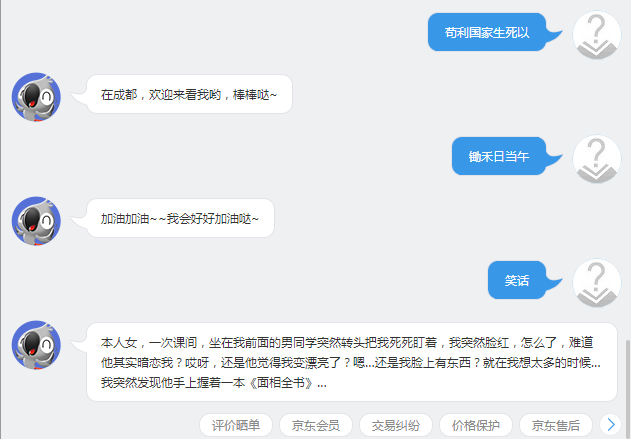
\includegraphics[width=0.8\textwidth]{jimi_chat1.png}
    \caption{\label{figure:jimi_chat} 京东“JIMI”案例}
\end{figure*}

“JIMI”和“ALIME”均为检索式智能客服机器人,
通过表\ref{table:jimi-skill}和图\ref{figure:jimi_chat}
可推测出“JIMI”的工作原理和实现方式与“ALIME”类似。
根据表\ref{table:jimi-skill}中“提问完整”技巧可知,
“JIMI”相比“ALIME”缺失了一定的上文关联能力,且对输入要求更加苛刻。

功能上,“JIMI”比“ALIME”多出了包括“笑话”、“对诗”和“天气查询”的闲聊服务功能。
首先“天气查询”本质上并不属于聊天的范畴而属于较为简单不涉及复杂语义分析的检索功能;
其次,通过实际测试,如图\ref{figure:jimi_chat}可知,“JIMI”所提供的“笑话”和“对诗”能力亦不属于生成式对话系统。
“前者”需要顾客输入关键词“笑话”,系统随后从笑话知识库中随机抽取一段笑话抛出;
“后者”甚至不能识别一些经典诗句,以致系统完全误解顾客意图。
因此“JIMI”的闲聊服务功能并不出彩,甚至给顾客造成了预期落差,产生了消极的对话体验。

虽然“JIMI”在对话窗体底部提供了“评价晒单”、“京东会员”、“交易纠纷”和“京东售后”等查询入口,
相比“ALIME”给顾客带来了一定程度的便利。
但这些入口严格意义上并不属于本文所研究的客服问答系统,因此不归为京东“JIMI”的优势功能。

\subsection{七鱼}
\label{subsection:qiyu}

网易“七鱼”是网易研发服务企业的检索式智能问答系统。其应用场景亦与“ALIME”和“JIMI”类似,
于2016年4月上线。
“七鱼”与“ALIME”、“JIMI”同为检索式问答系统。通过企业自建的知识库和相似词库完成关键词抽取和语义识别,
如图\ref{figure:wyqy_kd}所示。
\begin{figure*}[!htp]
    \centering
    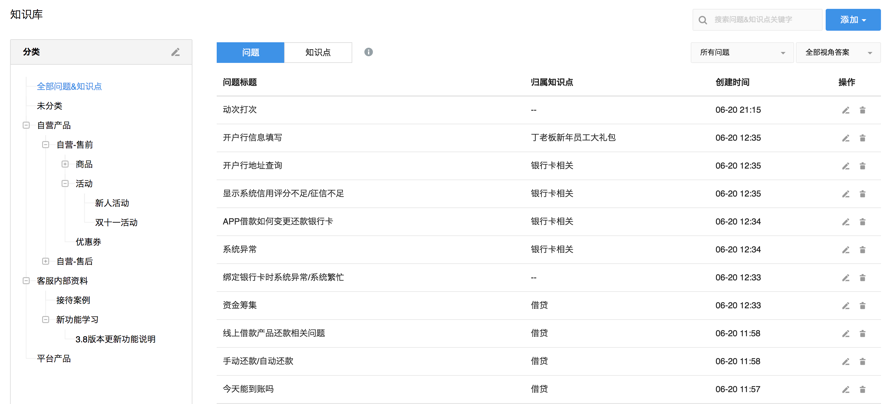
\includegraphics[width=\textwidth]{wyqy_kd.png}
    \caption{\label{figure:wyqy_kd} 网易“七鱼”知识库}
\end{figure*}

网易“七鱼”作为国内智能客服问答领域新生产品的代表,同样采取问题-知识检索的方式构建智能问答系统。
相较于“ALIME”、“JIMI”,“七鱼”采用开放网站、APP和微信接口的方式获取企业用户\wordnote{
    \url{https://github.com/qiyukf}
},
然而这种渠道优势如同“JIMI”查询入口亦不属于问答系统的原理范畴,因此同样不归为其优势功能。

\subsection{评价指标}
\label{subsection:evaluation}

目前由美国国家标准技术句主持的文本检索会议(TREC)
针对TREC/QA任务下的问答系统提出了一套评价指标\citep{voorhees2000building}。
该套评价指标针对不同类别问题略有不同,总体由3个部分组成,
实例查询准确率(Instance Precision)、实例查询召回率(Instance Recall)和F值(F1 Measures)。
其中,实例查询准确率指的是问答系统给出的正确答案占给出的全部答案的比例,
实例查询召回率指的是问答系统给出的正确答案的数量占所有正确答案的比例,F值则是实例查询准确率和实例查询召回率的调和平均值。
然而这套评价指标并不完全符合客服问答系统。

企业作为客服问答系统的使用者, 核心需求为保持和扩展顾客群体,进而提高盈利。
当然,反馈给顾客正确的应答毫无疑问为非常重要的问答系统评价指标,
然而在企业的需求下,在无法给予顾客准确应答的情况时,给予顾客以适当的情感抚慰,也有可能挽留顾客并满足顾客的情感需求。
顾客作为客服问答系统的参与主体,不局限于答案准确率,同时希望在快速获取准确答案的同时感受类人的交互。
因此应当考虑建立时间分数和智能客服类人程度的评价标准。

时间分数是客服回答机器人与顾客对话时间的分数。顾客和企业都希望能够以尽量短的时间得到(给出)正确的答案。
此处的时间可定义为对话时长或交互次数。对话时长目前主要受客户打字速度或其他因素的影响,若采用对话时长作为时间的评价标准,
则会产生相比交互次数更大的误差,因此以在顾客最终得到正确答案时客户回答机器人与顾客对话的交互次数作为时间分数的影响因素。
在顾客得到正确答案时,交互次数越少,时间分数越高,反之,交互次数越多,时间分数越低;在顾客无法得到正确答案时,时间分数为0。

知名的机器类人程度评价有“图灵测试”。
若在智能客服问答系统中建立图灵测试,
则需要取消问答系统中转接人工客服的功能并对顾客进行一定的误导以使顾客无法先验客服身份,
但此方法代价颇高。
由于自然语言的天然复杂性,现阶段的客服问答系统均无法达到较高的人类自然语言相似度。
机器无法理解自然语言表述导致无法抛出正确应答,顾客又无法转接人工客服,极易使顾客失去耐心和信任,造成顾客流失,
而这正是企业最不愿发生的。
因此图灵测试不适合直接应用与智能客服的类人评价。具体如何建立一套合理和有效的类人评价方法,值得学界和业界的继续探讨。

综上所述,本文借鉴TREC/QA评价体系,根据智能客服问答系统情景综合考虑了问答系统的应答质量、时间和类人程度因素,
提出了准确率、召回率、F值、时间分数和类人程度五元的综合评价体系。
其中,
准确率为问答系统给出的正确答案占给出的全部答案的比例;
召回率为问答系统给出的正确答案的数量占所有正确答案的比例;
F值为准确率和召回率的调和平均值;
时间分数为问答系统与顾客交互次数的函数;
类人程度是问答系统应答与人工客服应答的相似程度。

\subsection{系统对比}

由于缺乏相应训练集、测试集、知识库和完整评价指标,故此小节未完成...
    \section{混合智能问答系统}
\zihao{-4}
\label{section:mixed-system}

\subsection{意图识别}
\label{subsection:task-recognition}

如节\ref{section:peer-system}中所述,在线呼叫中心的客服领域普遍采用的是检索式智能问答系统。
该系统首先对顾客问题进行语法、语义分析,抽取关键词的组合,通过进行关键词组合的扩展确定问题类别和顾客问题意图;
然后连接本地/网络知识库对顾客意图进行检索,抛出补全信息请求应答或确定候选结果集;
接着对候选结果集进行排序,获取分值或概率最高的结果,将结果信息进行整合,抛出最终应答。

对于检索式智能问答系统,正确识别顾客问题意图是后续检索和反馈正确应答的关键。
目前的意图识别主要依赖问答系统用户即商家连接或自建的问题词库,根据该词库抽取关键词进而汇集关键词的组合完成意图识别。
在此过程中,往往会出现由于用户输入错字导致关键词抽取失败,或是长问句内包含多个问题以致无法准确
完成意图识别。

对于用户输入错字的问题,
由于基于词库或词典抽取关键词的特性,如果词库中没有包含错别字的组合,如表\ref{table:jimi-skill}中所举“优汇劵”和“优惠卷”,
词库包含“优惠卷”而不包含“优汇劵”,顾客若输入“优汇劵”则导致关键词“优惠卷”失败,无法完成意图识别。

值得注意的是,在输入错字的情况下,由于汉语拼写和输入的特性,一些规律是可以被归纳和利用的。
顾客输入的错误关键词和正确关键词往往是拼音相同或相近的,这种相同和相近在一定程度上反映了错误关键词和正确关键词的距离。
而传统的文本分聚类往往忽视了拼音上的距离,
仅考虑词在整个文档或训练集中出现的频率并将这种统计信息转化为词向量权值,如TF-IDF方法,
训练集样本本身对此方法有较大影响,易出现拟合,降低模型的泛化能力。
单纯考虑错误关键词与正确关键词的拼音相似度也是不可取的,对于多字组合的关键词,其拼音完全相似的词集数为字各自拼音完全相似的词集数之积,
因此综合考虑词的统计信息与拼音相似度作为其向量权值是一种预期效果较优的向量化方法。

在明确了词向量化方法后,此时关键词的识别可转化为对应不同关键词的多分(聚)类问题,完成知识库(词库)的扩充,实现关键词的识别。
通过结合关键词的句法依存结构分析\citep{问题识别},完成长文句内多问题的切分,进而实现用户输入错字下和长问句下的意图识别。

\subsection{端到端学习}

基于检索式问答系统一般针对用户的自然语言问句,提供准确的应答。
例如,对于问句“泰戈尔的出生地在哪儿?”,返回“加尔各答”。
但是,仅仅提供这种孤零零的答案实体并不是非常友好的交互方式,用户更希望接受类人的回答,
如以自然语言表示的完整答案(以下简称自然应答),“印度诗人泰戈尔出生于加尔各答市”。

单纯生成自然应答的生成式问答系统往往被应用在无任务驱动的聊天场景。
在这种场景下,用户没有明确的目标,不需要获取某种准确的信息,因此很少涉及到对知识库的检索。
如何检索知识库中的已有知识生成能够准确问答问题且流利的自然应答是一种挑战。

\begin{figure*}[!htp]
    \centering
    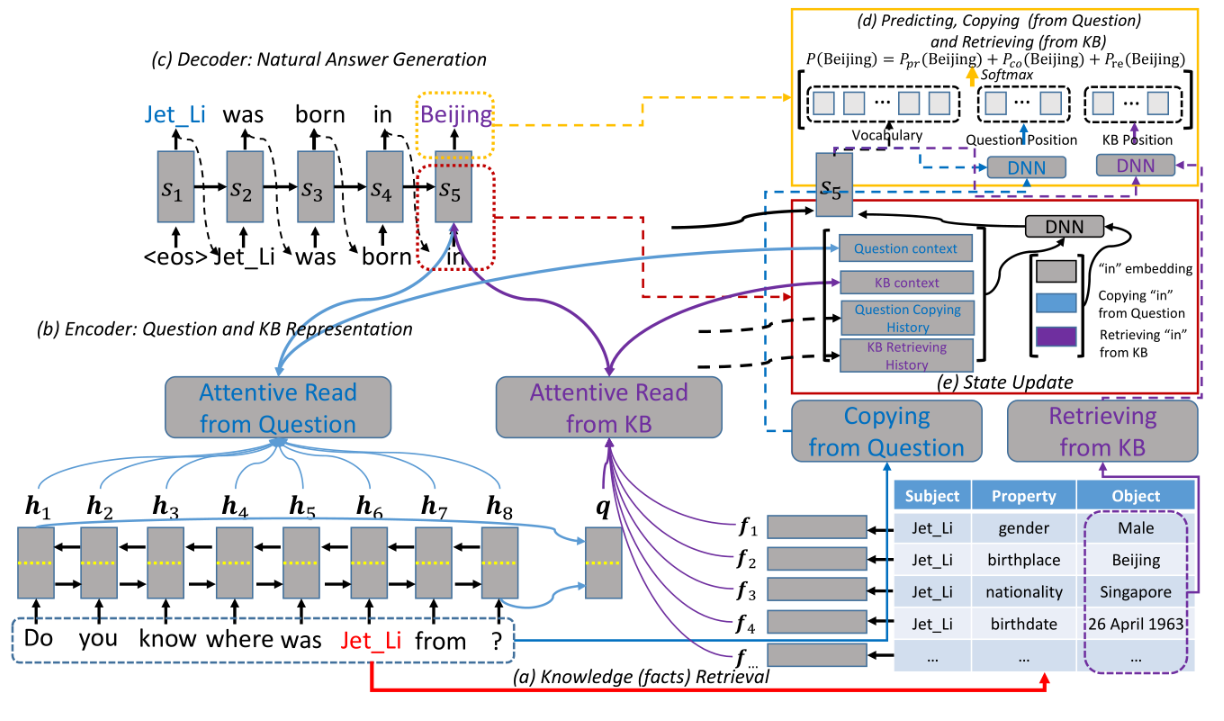
\includegraphics[width=0.8\textwidth]{mixed_system.png}
    \caption{\label{figure:mixed_system} 自然答案生成系统}
\end{figure*}
为解决此问题,中科院自动化所的何世柱博士等\citep{hegenerating}提出了一个端到端的问答系统。
如图\ref{figure:mixed_system}中“Do you know where was Jet Li from?”为例进行阐述。

首先对问句进行语义分析,抽取出关键词,连接知识库进行检索,获取到与李连杰相关的知识实体;
然后基于双向循环神经网络Bi-RNN的Encoder-Decoder机制对问句进行问题编码,
对知识库检索结果进行知识编码;
接着根据问题和知识的编码向量来生成自然答案。
自然答案虽然是词序列,但是不同的词可能需要通过不同途径获得。
例如,对于上述问题的答案“Jet Li was born in Beijing”,
词语“Jet Li ”需要从源问句中拷贝得到,实体词“Beijing”需要从知识库中检索得到,
而其他词如“born”、“in”等需要通过模型预测得到。
因此,这里在标准的序列到序列(Sequence-to-Sequence)模型基础上,
融合了三种词语获得模式(包括拷贝、检索和预测),
用统一的模型对其建模,
让各种模式之间相互竞争相互影响,
最终对问题生成一个最优的自然答案。

值得注意的是,该模型一方面仅以当前语句进行Encoder没有考虑上下文,无法进行上下文关联。
另一方面,由于关键词是问句中抽取,相关直接从知识库中直接拷贝,若输入错别字,则同样会造成生成失败的情况。
因此改模型可从两方面进行改进,一是结合小节\ref{subsection:task-recognition}中的意图识别方法,对关键词词库进行扩充,
实现关键词的正确抽取;二是考虑多轮对话情景,引入Gated RNN Unit对进行上文记忆和下文推演,以生成更好的自然语言应答。
    % \section*{文献摘要}
大多数人与人之间的对话发生在半合作环境中,具有不同目标的代理人试图通过谈判就决策达成一致。
虽然谈判需要复杂的沟通和推理技巧,但谈判的结果很容易区分,即``成功-失败''。
如何进行谈判对于AI来说是一个很有趣的问题。

Facebook Artificial Intelligence Research(以下简称FAIR)就此问题收集了一个关于多项目谈判任务的
人与人之间(以下简称``人-人'')的对话数据集,
建立了一个端到端学习(end to end learning)的模型训练机器进行谈判,并展示了谈判机器人的可能性。
    % \section{介绍}
\zihao{-4}

\label{section:introduction}
在进行谈判时,
智能代理\wordnote{
    Intelligent Agents,即从事谈判工作且具有一定智能的代理。
    论文中没有指定其必须为人类,因此在定义上智能代理可为机器或人类。
    }(以下简称代理)
通常需要与怀有不同目标的他人合作,谈判的过程通常以自然语言为主题的对话来体现。
具体来说,谈判是一个以自然语言为载体,通过推理与对话,最终达成或无法达成自己意图的过程。
其中,谈判的资源为总数为5-7的书、帽子和球三种资源项目;主体为两位智能代理;
价值函数\wordnote{
    Value Function,即项目的价值函数。
    资源项目的总价值为10分,各项目单位价值为非负整数。
    项目价值函数在各智能代理处为随机生成,且在谈判前两位代理互不了解对方的价值函数
    因此会出现某些谈判中某资源项目对两位代理具有相同的价值,
    这也更接近现实。
}
为对于给定的资源项目均有且只有唯一对应的价值;意图为通过对话使最终自己取得的资源价值最大,即文中所述``goals"。
这样的过程要求代理能够理解、推理和通过语言表述来实现意图。

FAIR以概率的形式描述代理在谈判中的行为,通过选取最大的行为概率来推理谈判行为,
并以此构建了一个端到端的神经网络模型训练机器进行谈判。
FAIR首先建立了似然模型\wordnote{
    Likelihood Model,对应论文Section 3。
},
通过循环神经网络监督学习\quotes{人-人}谈判数据,
使机器模仿人在谈判中的语言以达成交易;
随后发现这种方法会导致机器为了达成交易不考虑自身意图,即过于妥协。
因此,FAIR在此之上提出了加强学习\wordnote{
    Goal-based Training,对应论文Section 4。
}
和对话推演\wordnote{
    Goal-based Decoding,对应论文Section 5。
}
两种模型优化机器的谈判能力,使其实现意图,而不仅是模仿对话达成交易。

FAIR针对所提的三种模型提出了自己的评价指标\wordnote{
    Comparison Systems,对应Section 6。
}:分数、成交率和帕累托最优率。
原因经我归纳有三,一是本文虽使用了统计机器翻译(SMT)模型的方法,但侧重于实现用于谈判的AI,
因此SMT的Blue Score评价指标在此并不适用;二是本文对谈判过程进行了输入-对话-输出的表述,
其中对输入中的项目建立了价值函数,,对输出进行了成交-失败区分,
故因此可得输出价值分数与成交率,所以在此提出了分数和成交率;
三是在两人谈判模型中,不同的输出对应不同价值分数,这是一个可帕累托改善过程,
故因此提出了帕累托最优率。
    % \section{数据收集}
\zihao{-4}
\label{section:data_collection}

FAIR利用Amazon Mechanical Turk进行了两人间多项目谈判的自然语言数据收集任务,共收集了5808个对话数据集。
在本篇论文中,FAIR对于\quotes{两人间多项目谈判}的定义引用于\citet{Fershtman-4,DevaultMell-5},
若不实现阅读这两篇参考文献,读者很容易对谈判产生误解,误解为两位代理需要通过谈判交易对方的资源。
实际上,在该谈判下,项目为两位代理要瓜分的资源,价值为随机生成;
用户即代理仅知道自己的项目价值,另外一个代理的项目价值函数需要通过对话推理得出;
输出为用户通过谈判结果所认为自己所应该得到项目部分。

值得注意的是,
谈判结果可以为成交即\quotes{Deal},也可以为失败即\quotes{No Deal},
那么如何确定谈判结果的标的?
如项目和输出的定义,若谈判成交,则两位用户输出的各项目之和应当分别等于各项目总数。
因此,FAIR在本文中以\quotes{输出的各项目之和应当分别等于各项目总数}作为谈判结果的标的。

\begin{figure*}[ht]
\centering
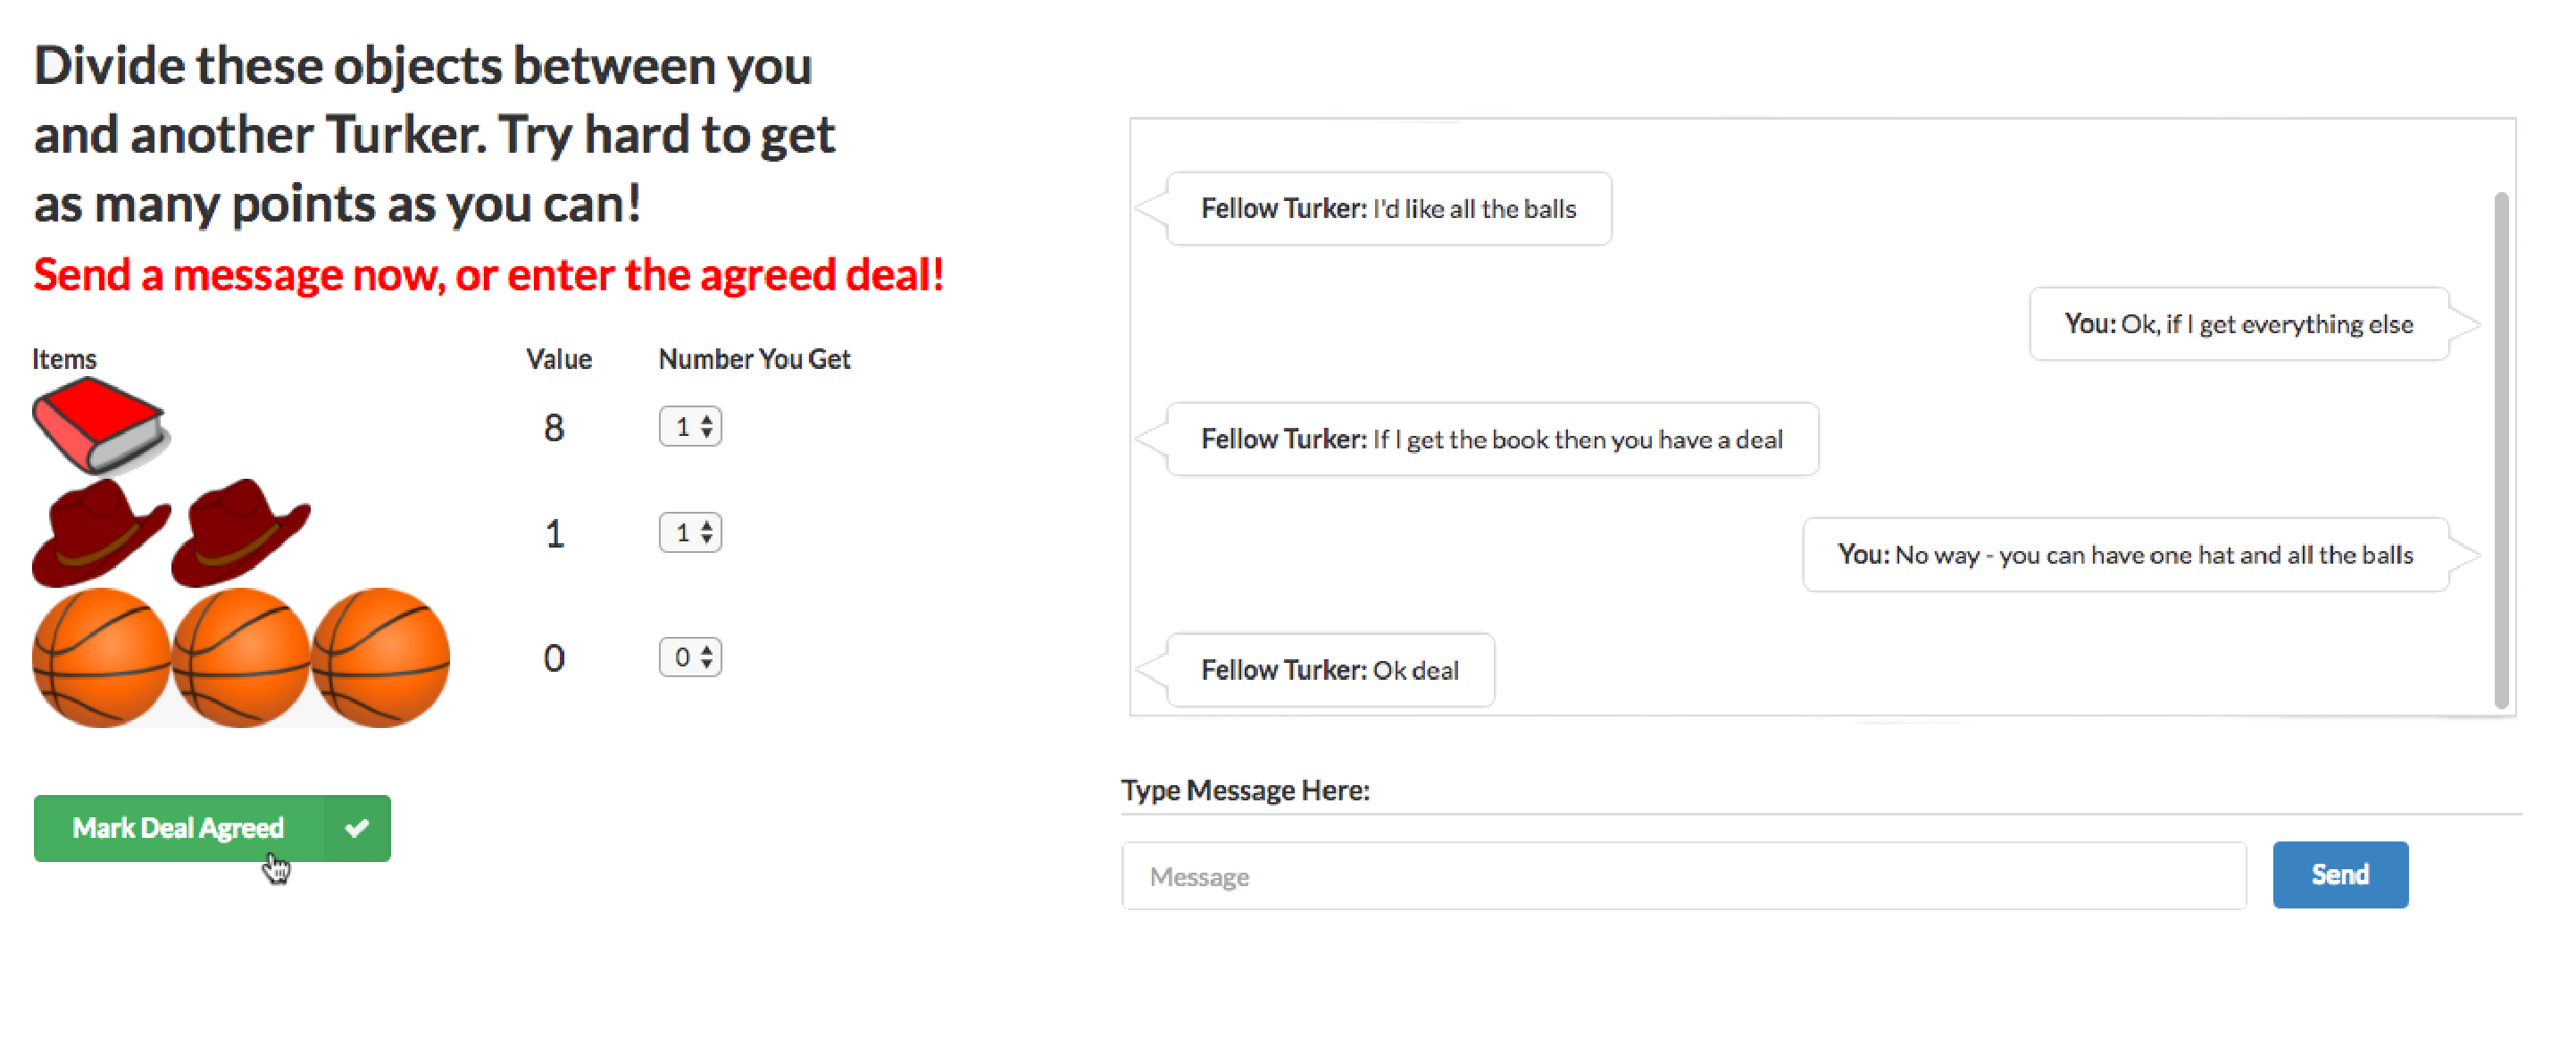
\includegraphics[width=\textwidth]{example_negotiation.eps}
  \vspace{-4.0em}
\caption{\label{figure:turk}谈判对话采集界面,FAIR用其收集\quotes{人-人}谈判文本数据集}
\end{figure*}
FAIR在\citet{DasKottur-6}的基础上建立谈判数据采集界面。
如图\ref{figure:turk}所示,在进行数据采集时,界面会显示各项目的数量、价值、输出\wordnote{
    Output,即输出,表示代理经过对话后认为自己应该取得的各项目数量。
}和对话。
其中,书、帽子和球的数量以Items下的图标数量表示,价值以Values下的数值表示,
输出以Number You Get下的数值表示,对话以对话框形式表述和记录。
以图\ref{figure:turk}为例,项目的数量分别为1、2和3,
价值分别为8、1和0,输出分别为1、1和0,对话记录如对话框所示。
    % \section{似然模型}
\zihao{-4}

\label{section:likelihood}

FAIR在本节中提出了一个谈判的基准模型。
作为基准模型,机器至少应能根据输入的项目及其价值模仿人进行谈判。
在此,首先对谈判过程和主体行动进行结构化的分析。
\begin{figure*}[ht!]
\centering
\newcommand{\turnA}{I want the books and the hats, you get the ball}
\newcommand{\turnB}{Give me a book too and we have a deal}
\newcommand{\turnC}{Ok, deal}
\newcommand{\turnD}{\textless choose\textgreater}
\newcommand{\choiceA}{2x\textit{book} 2x\textit{hat}}
\newcommand{\choiceB}{1x\textit{book} 1x\textit{ball}}

\newcommand{\itemvalue}[3]{#2x\textit{#1} & \textit{value}=#3}
\newcommand{\bookA}{\itemvalue{book}{3}{1}}
\newcommand{\hatA}{\itemvalue{hat}{2}{3}}
\newcommand{\ballA}{\itemvalue{ball}{1}{1}}

\newcommand{\bookB}{\itemvalue{book}{3}{2}}
\newcommand{\hatB}{\itemvalue{hat}{2}{1}}
\newcommand{\ballB}{\itemvalue{ball}{1}{2}}

\newcommand{\goals}[3]{
\setlength{\tabcolsep}{0.2em} % for the horizontal padding
\begin{tabular}{ll}
     #1\\#2\\#3
\end{tabular}
}


\tikzstyle{arrow} = [thick,->]
\tikzset{>=latex}

\begin{tikzpicture} 
  \tikzstyle{box} = [rectangle, rounded corners, font=\sffamily\footnotesize, text width=2.45cm, draw=black]
  
  
      \node [box, draw=black, thick, fill = white, minimum width = 6.7cm, minimum height = 8cm]  at (current page.north west) (raw)
    {};
    
    \node[below right] at (raw.north west) (rawlabel) {\underline{\bfseries Crowd Sourced Dialogue
}};
    
  
    \node [box, fill=blue!30, text width      = 2.45cm, below=0.0cm of rawlabel.south west, anchor=north west, xshift=0.2cm]
    (User1Goals)
    {\underline{\bfseries Agent 1 Input}\\
      \goals{\bookA}{\hatA}{\ballA}   
     };
     
    \node [box, right = 0.8cm of User1Goals, fill = blue!30, text width      = 2.45cm]
    (User2Goals)
    {\underline{\bfseries Agent 2 Input}\\
      \goals{\bookB}{\hatB}{\ballB}   
    };
      
    \node [box, below = 0.9cm of User1Goals.south west, anchor=north west, fill = yellow, text width      = 6cm]
    (Dialog)
    {\underline{\bfseries Dialogue}\\
      \textbf{Agent 1:} \turnA\\
      \textbf{Agent 2:} \turnB\\
      \textbf{Agent 1:} \turnC\\
      \textbf{Agent 2:} \turnD\\

    }; 
    
    \node [box, below = 0.8cm of Dialog.south west, anchor=north west, fill = red!30, text width=2.3cm]
    (User1Choice)
    {\underline{\bfseries Agent 1 Output}\\
      \choiceA\\      
    };

    \node [box, right = 1.2cm of User1Choice, fill = red!30, text width=2.3cm]
    (User2Choice)
    {\underline{\bfseries Agent 2 Output}\\
      \choiceB\\      
    };


    \node [box, right = 1cm of raw.north east, ,anchor=north west, draw=black, thick, fill = white, minimum width = 8cm, minimum height = 3.75cm] (perspective1)
    {};
    
    
    \draw [arrow] (User1Goals) -- (Dialog);
    \draw [arrow] (User2Goals) -- (Dialog);
    \draw [arrow] (Dialog) -- (User1Choice);
    \draw [arrow] (Dialog) -- (User2Choice);

    
    
    \node[below right] at (perspective1.north west) (perspective1label) {\underline{\bfseries Perspective: Agent 1}};


    \node [box, below = 0.5cm of perspective1, draw=black, thick, fill = white, minimum width = 8cm, minimum height = 3.75cm] (perspective2)
    {};
    
    \node[below right] at (perspective2.north west) (perspective2label) {\underline{\bfseries Perspective: Agent 2}};


    \node [box, fill = blue!30, text width      = 2.45cm, below=0.0cm of perspective1label.south west, anchor=north west, xshift=0.2cm]
    (perspective1_goals)
    {\underline{\bfseries Input}\\
      \goals{\bookA}{\hatA}{\ballA}   
     };
     
         \node [box, fill = red!30, text width      = 2.45cm, below = 0.2cm of perspective1_goals]
    (perspective1_choice)
    {\underline{\bfseries Output}\\
      \choiceA\\      
     };

    \node [box, right = 1cm of perspective1_goals.north east, anchor=north west, fill = yellow, text width      = 3.5cm]
    (perspective1_dialog)
    {\underline{\bfseries Dialogue}\\
      \textbf{write:} \turnA\ \textbf{read:} \turnB\ 
      \textbf{write:} \turnC\ \textbf{read:} \turnD
    }; 
    
        \node [box, fill = blue!30, text width      = 2.45cm, below=0.0cm of perspective2label.south west, anchor=north west, xshift=0.2cm]
    (perspective2_goals)
    {\underline{\bfseries Input}\\
      \goals{\bookB}{\hatB}{\ballB}   
     };
    
        \node [box, right = 1cm of perspective2_goals.north east, anchor=north west, fill = yellow, text width      = 3.5cm]
    (perspective2_dialog)
    {\underline{\bfseries Dialogue}\\
      \textbf{read:} \turnA\ 
      \textbf{write:} \turnB\ 
      \textbf{read:} \turnC\ 
      \textbf{write:} \turnD
    }; 
    
             \node [box, fill = red!30, text width      = 2.45cm, below = 0.2cm of perspective2_goals]
    (perspective2_choice)
    {\underline{\bfseries Output}\\
      \choiceB\\      
     };
    
    \draw [arrow] (perspective1_goals) -- (perspective1_dialog);
    \draw [arrow] (perspective2_goals) -- (perspective2_dialog);

    \draw [arrow] (perspective1_dialog) -- (perspective1_choice.east);
    \draw [arrow] (perspective2_dialog) -- (perspective2_choice.east);
\end{tikzpicture}
\caption{\label{figure:representation} 谈判过程展示 }
\end{figure*}


\subsection{Date Representation}
\label{subsection:date_representation}

模型将各项目数量、各代理的价值函数作为输入,表示为input goal $\vec{g}$,
其中$\vec{g}$由6个非负整数组成,依次对应各项目的数量和价值;
将代理间的对话作为中间过程,表示为对话dialogue $\vec{x}$,
其中tokens $x_{0..T}$表示对话$\vec{x}$中依次进行的对话;
将代理的输出作为模型输出,表示为output $\vec{o}$,
其中$\vec{o}$由6个非负整数组成,表示三种项目分配给两位代理的数量。

以图\ref{figure:representation}为例,
从每个代理的角度将对话(图\ref{figure:representation}左)分为了两个对话示例(图\ref{figure:representation}右)。

模型的输入为:3本书、2顶帽子、1个球和各代理的价值函数。
其中,对于代理1即\quotes{Agent 1},各项目的单位价值分数分别为:1、3和1,即输入为\quotes{3 1 2 3 1 1};
对于代理2即\quotes{Agent 2},各项目的单位价值分数分别为:2、1和2,即输入为\quotes{3 2 2 1 1 2};
对于每一位代理,因谈判的目的是瓜分资源而不是交易资源,所以输入项目相同且项目总数在5-7之间,项目价值总分均为10。

模型的中间过程根据代理的不同,划分为了两种情况。
其中,对于代理1,首句行为为写\quotes{write},对于代理2,首句行为为读\quotes{read}。

模型的输出为\quotes{2 2 0 1 0 1}。
其中前三位整数\quotes{2 2 0}表示代理1通过谈判认为自己可取得的项目数量,即2本书和2顶帽子;
后三位整数\quotes{1 0 1}表示代理2通过谈判认为自己可取得的项目数量,即1本书和1个球。

值得注意的是,在图\ref{figure:representation}中,因为两个代理输出中各项目选择加起来等于各项目总数,
因此图\ref{figure:representation}中的谈判视为达成,即\quotes{Deal}。
若出现两个代理输出中各项目选择加起来不等于各项目总数,如输出为\quotes{3 2 0 1 0 1},
则表示谈判失败,即\quotes{No Deal}。

\subsection{GRUs RNN}
\label{subsection:grus_rnn}

FAIR在本节中,提出了一个序列-序列网络,以根据代理的输入产生代理的对话,如图\ref{figure:model:supervised}。

模型使用了\citet{  Cho-18,  Cho-28}中提出的循环神经网络,即\quotes{recurrent neural network},
并借鉴了其文章中所提出的\quotes{RNN Encoding-Decoding}机制。
该机制作为此篇论文处理对话自然语言的基础,且文中并未介绍,因此有必要在此就其关键概念进行阐述。
\begin{figure*}[ht!]
    \centering
    \begin{minipage}{0.5\textwidth}
        \centering
        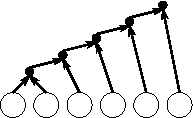
\includegraphics[width=0.5\textwidth]{rnn.pdf}
        \subcaption{\label{figure:rnn} RNN}
    \end{minipage}%
    \begin{minipage}{0.5\textwidth}
        \centering
        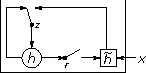
\includegraphics[width=0.5\textwidth]{hidden_unit.pdf}
        \subcaption{\label{figure:gated_unit} Gated Recurrent Unit}
    \end{minipage}%
    \caption{\label{figure:gated_rnn} GRUs RNN}
\end{figure*}

不同于传统的FNN(Feed-forward Neural Networks,前向反馈神经网络),
RNN引入了循环来处理序列数据。典型的序列数据如文本,由一定顺序组成的词构成。
在传统的神经网络模型中,从输入层到隐藏层再到输出层,层与层之间为全连接,但每层之间的节点是无连接的。
这种简单的神经网络对于很多问题无能为力,以翻译模型为例,要预测输出句子即输出词的组合,
需要考虑上文甚至上下文的情景,因为句子中的前后单词并不是独立的。

RNN之所以称为循环神经网络,是因其序列的当前输出与前面的输出有关,如图\ref{figure:rnn}所示。
具体表现形式为,网络会通过激活函数和误差传递对前面的信息进行记忆并应用至当前输出的计算中,
即隐藏层之间的节点不再无连接而是有连接的。
如对于可变长度序列$\vx=(x_1, \dots, x_T)$,对于每一步$t$,隐藏层单元$\vh_{\qt{t}}$的更新公式为:
\begin{equation}
    \label{eq:rnn_hidden_unit_update}
    \vh_{\qt{t}} = f\left( \vh_{\qt{t-1}}, x_t \right)
\end{equation}

其中$f$为非线性激活函数。通过将词的预测转化为词概率的计算问题,
RNN可以通过学习预测出下一个输出的所有词的概率,通过选择概率最大的词完成预测。
如共有$K$个词,则第$t$个词$x_{t,j}$的计算公式为:
\begin{equation}
    \label{eq:rnn_word_prediction}
    p(x_{t,j} = 1 \mid x_{t-1}, \dots, x_1) = \frac{\exp \left(
        \vw_j \vh_{\qt{t}}\right) } {\sum_{j'=1}^{K} \exp \left( \vw_{j'}
        \vh_{\qt{t}}\right) }
\end{equation}

其中$j$表示所有可能的词,$j=1,\dots,K$,
$\vw_j$是词权重矩阵$\mW$的列。
通过组合词的概率,从而完成词序列$\vx$的预测。
\begin{equation}
    % \label{eq:distribution}
    p(\vx) = \prod_{t=1}^T p(x_t \mid x_{t-1}, \dots, x_1)
\end{equation}

因为这一特性,RNN及其改进型被广泛应用于机器翻译模型中。
\citet{  Cho-28}在此基础上提出了适用于统计机器翻译的词嵌入方法与Encoder-Decoder机制,
如图\ref{figure:rnn_encdec}。
\begin{figure*}[ht!]
    \centering
    \begin{minipage}{0.4\textwidth}
        \centering
        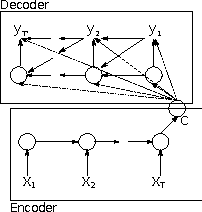
\includegraphics[width=0.4\textwidth]{unit_encdec.pdf}
        \subcaption{\label{figure:unit_encdec} Units Encode-Decode}
    \end{minipage}%
    \begin{minipage}{0.6\textwidth}
        \centering
        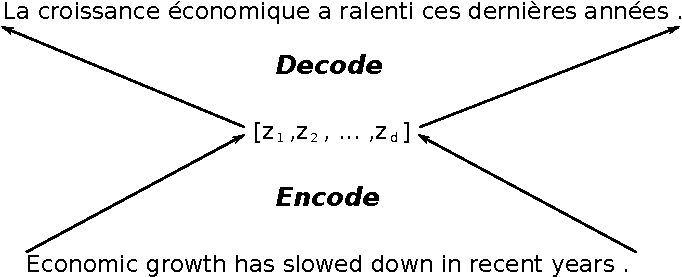
\includegraphics[width=0.6\textwidth]{seq_encdec.pdf}
        \subcaption{\label{figure:seq_encdec} Sequence Encode-Decode}
    \end{minipage}%
    \caption{\label{figure:rnn_encdec} RNN Encode-Decode}
\end{figure*}
在现实情况下,序列数据的输入一般都是可变长度的。
图\ref{figure:unit_encdec}展示了将可变长度的序列数据$\vx=(x_1, \dots, x_T)$作为输入嵌入至矩阵$c$,
然后再以$c$和目标序列数据$\vy=(y_1, \dots, y_{T-1'})$作为输入,生成$\vy=(y_1, \dots, y_{T'})$。

值得注意的是,这里的$T$和$T'$可能是不同的。

此时,隐藏层单元$\vh_{\qt{t}}$的更新公式为:
\begin{equation}
    % \label{eq:decode_hidden_unit_update}
    \vh_{\qt{t}} = f\left( \vh_{\qt{t-1}}, y_{t-1}, \vc \right)
\end{equation}

同样的,目标词$y_t$的计算公式为:
\begin{equation}
    P(y_t | y_{t-1}, y_{t-2}, \ldots, y_1, \vc) = g\left(\vh_{\qt{t}}, y_{t-1}, \vc \right)
\end{equation}


理论上,RNN能对任何长度的序列数据进行处理,但是由于梯度消失和梯度爆炸问题,
实际运用中多使用改进型RNN,如图\ref{figure:gated_unit}所示,便是Gated Recurrent Unit(GRU)。
结合GRU的改进型Gated Recurrent Units RNN即为此篇论文所使用GRUs。

以图\ref{figure:gated_unit}和图\ref{figure:seq_encdec}为例。
以$x=(\vx_1, \vx_2, \cdots, \vx_T)$表示输入的序列数据,其中$\vx_t \in\RR^d$。
GRUs由四个权重矩阵组成,分别为$\mW^l$、$\mW^r$、 $\mG^l$和$\mG^r$。
对于任意一步$t \in \left[ 1, T-1\right]$,第$j$个隐藏层单元$h^{(t)}_j$计算为:
\begin{equation}
    % \label{eq:grconv_main}
    h^{(t)}_j = \omega_c \tilde{h}^{(t)}_j + \omega_l h^{(t-1)}_{j-1} + \omega_r h^{(t-1)}_j
\end{equation}

其中$\omega_c$、$\omega_l$和$\omega_r$值的和为$1$。隐藏层单元初始化为:
\begin{equation}
    h^{(0)}_j = \mU \vx_j
\end{equation}

其中$\mU$表示输入数据的隐藏层映射矩阵。

新的激活函数$\tilde{h}^{(t)}_j$计算为:
\begin{equation}
    \tilde{h}^{(t)}_j = \phi\left( \mW^l h^{(t)}_{j-1} + \mW^r h^{(t)}_{j}
    \right),
\end{equation}

其中$\phi$为非线性激活函数。

聚集系数$\omega$计算为:
\begin{equation}
    \left[ 
        \begin{array}{c}
            \omega_c \\
            \omega_l \\
            \omega_r
        \end{array}
    \right] = \frac{1}{Z}
    \exp\left( \mG^l h^{(t)}_{j-1} + \mG^r h^{(t)}_{j}
    \right)
\end{equation}

其中$\mG^l, \mG^r \in \RR^{3 \times d}$且
\begin{equation}
    Z = \sum_{k=1}^3 \left[\exp\left( \mG^l h^{(t)}_{j-1} + \mG^r h^{(t)}_{j} \right)\right]_k.
\end{equation}

由此完成了基于GRUs RNN的词嵌入与Encode-Decode机制。
\citet{  Cho-18,  Cho-28}利用该机制实现了一个英译法的统计机器翻译模型。

\subsection{Supervied Learning}
\label{subsection:supervised_learning}

如\ref{subsection:grus_rnn}中所提,FAIR在本小节中,提出了一个序列-序列网络,以根据代理的输入产生代理的输出。
其中,
该序列-序列网络,或称为端到端网络,是在\citet{  Cho-18,  Cho-28}所提的GRUs RNN Encode-Decode基础上的应用与改进\wordnote{
    与\citet{  Cho-18,  Cho-28}相同的是,此篇论文的对话输入和输出也均是文本序列数据;
    不同在于,此篇论文的输入中包含了项目数量和价值,并希望最终输出取得最大的价值分数,而不仅是流畅地进行谈判对话。
};
代理的输入包含初始项目数量、价值和对话;
代理的输出包含对话和选择。

因此此篇论文所提的端到端网络模型使用了四个RNN:
$\text{GRU}_w$,$\text{GRU}_g$,$\text{GRU}_{\overrightarrow{o}}$和$\text{GRU}_{\overleftarrow{o}}$。

\def\layersep{1.0cm}
%\newcommand{\counts}[2]{\textit{#2x}\textbf{#1}}
\newcommand{\counts}[2]{\textbf{#1} \textit{count}=#2}
\newcommand{\values}[2]{\textbf{#1} \textit{value}=#2}


\def\goals{}%\counts{book}{3}, \values{book}{2}, \counts{hat}{2}, \values{hat}{1}, \counts{ball}{1}, \values{ball}{2}, \values{ball}{2}}

    \tikzstyle{every pin edge}=[<-,shorten <=1pt]
    \tikzstyle{neuron}=[circle,fill=black!25,minimum size=17pt,inner sep=0pt]
    \tikzstyle{input neuron}=[neuron,draw=black!50, fill=white]
    \tikzstyle{output neuron}=[neuron, fill=red!50]
    \tikzstyle{hidden neuron}=[neuron, fill=blue!50]
    \tikzstyle{annot} = [text width=4em, text centered]
  \tikzstyle{box} = [rectangle, rounded corners, font=\sffamily\footnotesize, text width=2.3cm, draw=black]

\newcommand{\network}[0]{
\scalebox{0.7}{
\begin{tikzpicture}[shorten >=1pt,->,draw=black!50, node distance=\layersep]
\tikzset{>=latex}

  
  
      \node [box, draw=black, thick, fill = white%, minimum width = 2.7cm, minimum height = 1cm
      ] at (2,0.2) (enc) {Input Encoder};

      \node [box, draw=black, thick, fill = white%, minimum width = 2.7cm, minimum height = 1cm
      , right = 1cm of enc]  (dec) {Output Decoder};

   

    \foreach[count=\y,evaluate=\y as \prevx using int(\y-2)] \name in \words {
        \node[input neuron] (H-\y) at (\prevx, -2) {};
        \node[anchor=base] (O-\y) at (\prevx, -3) {\name};
    }

    \foreach[count=\y,evaluate=\y as \prevx using int(\y-1)] \w in \written {
        \ifthenelse{\y>1}{\path (O-\prevx) edge (H-\y);}{}
        \ifthenelse{\y>1}{\path (H-\prevx) edge (H-\y);}{}
        \ifthenelse{\y>0 \AND \w=1}{\path (H-\y) edge (O-\y);}{}
        

        \path (enc) edge (H-\y);
        \path (H-\y) edge (dec);
    }


%[evaluate=\x as \evalx using int(\x+1)]
\end{tikzpicture}
}
}



\begin{figure*}[t!]
    \def\words{\you,\vphantom{.}\space\space Take, one, hat, \them, I, need, two, \you, deal, \dots}

    \centering
    \begin{subfigure}[t]{0.5\textwidth}
        \def\written{1, 1, 1, 1, 1, 1, 1, 1, 1, 1, 1}
        \centering
        \network
        \caption{\label{figure:model:supervised} Supervised Training}
    \end{subfigure}%
    ~ 
    \begin{subfigure}[t]{0.5\textwidth}
        \def\written{0, 1, 1, 1, 1, 0, 0, 0, 0, 1, 1}
        \centering
        \network
        \caption{\label{figure:model:reinforcement} Decoding, and Reinforcement Learning}
    \end{subfigure}
    \caption{\label{figure:model} 端到端神经网络}
\end{figure*}
代理的输入$\vec{g}$通过$\text{GRU}_g$进行Encode,对应的隐藏层单元为$h^g$。
模型基于$h^g$和$x_{t-1}$对$x_t$进行依次预测。
对于每一步$t$, $\text{GRU}_w$都将
上一隐藏层单元$h_{t-1}$、上一词$x_{t-1}$\wordnote{
    通过矩阵$E$进行词嵌入。
}和$h^g$
作为神经网络的输入,以更新当前的隐藏层单元$h_t$。
\begin{equation}
h_t = \text{GRU}_w(h_{t-1}, [Ex_{t-1}, h^g])
\end{equation}

因此,目标词$x_t$的计算关系为:
\begin{equation}
p_\theta (x_t | x_{0.. t-1}, \vec{g}) \propto \exp(E^T h_t)
\end{equation}

值得注意的是,此时的模型会同时预测两位代理的对话词,并且模型依然是前馈的。

在对话的最后,代理会输出选择,以$\vec{o}$表示。
在这里,模型对两位代理的选择通过相互独立的分类器独立预测\wordnote{
    这也是为什么要在\ref{subsection:date_representation}中需要对代理分开进行建立输入、中间过程和输出的原因。
}。
分类器通过对话共享双向$\text{GRU}_o$模型和Attention机制\citep{BaarslagFujita-17},
在对话和$\vec{g}$的基础上进行词预测。
\begin{align}
h^{\overrightarrow{o}}_t &= \text{GRU}_{\overrightarrow{o}}(h^{\overrightarrow{o}}_{t-1}, [Ex_{t}, h_t])\\
h^{\overleftarrow{o}}_t &= \text{GRU}_{\overleftarrow{o}}(h^{\overleftarrow{o}}_{t+1}, [Ex_{t}, h_t])\\
h^o_t&=[h^{\overleftarrow{o}}_t, h^{\overrightarrow{o}}_t]\\
h^a_t&=W[\tanh(W'h^o_t)]\\
\alpha_t &= \frac {\exp(w \cdot h^a_t)}{\sum_{t'} \exp(w\cdot h^a_{t'})}
\end{align}
\begin{equation}
h^s = \tanh(W^s[h^g, \sum_t \alpha_t h_t])
\end{equation}

最终的选择则在对话、$\vec{g}$和$h^s$的基础上预测,计算关系为:
\begin{equation}
p_\theta(o_i | x_{0..t}, \vec{g}) \propto \exp(W^{o_i} h^s)
\end{equation}

模型通过降低对话预测损失和选择预测损失来实现较好的预测效果。
两个误差间的权重通过$\alpha$来调节。
\begin{equation}
\label{eq:supervised}
L(\theta) = -\underbrace{\sum_{\vec{x},\vec{g}} \sum_{t} \log p_\theta(x_t | x_{0.. t-1}, \vec{g})}_{\text{Token prediction loss}} - \alpha \underbrace{\sum_{\vec{x},\vec{g},\vec{o}} \sum_{j} \log p_\theta(o_j | x_{0.. T}, \vec{g})}_{\text{Output choice prediction loss}}
\end{equation}

不同于\citet{VinyalsLe-19}的神经网络对话模型,FAIR的方法考虑和共享了读取和写入词的所有参数。

\subsection{Decoding}
\label{subsection:decoding}

在Decoding的过程中,模型必须要根据对话历史$x_{0..t-1}$和输入项目数量与价值$\vec{g}$产生$x_{0..T}$。
如同\ref{subsection:grus_rnn}中的Decode过程,也是通过选取最大概率词的方式进行预测。计算关系为:
\begin{equation}
 x_t \sim p_\theta(x_t | x_{0..t-1}, \vec{g})
\end{equation}

整个对话过程以任一一方代理写出结束标志词\wordnote{
    \emph{end-of-dialogue},即结束标志词,如\quotes{Deal}、\quotes{OK}和\quotes{Okey}等。
}时结束。这时模型预测出选择$\vec{o}$,具体为从满足约束条件的可行输出选择集$O$中选择概率最高的那个。
\begin{equation}
\label{equation:output}
\vec{o}^{*} = \argmax_{\vec{o}\in O} \prod_{i} p_\theta(o_i | x_{0.. T}, \vec{g})
\end{equation}

值得注意的是,此篇论文在这里使用了\quotes{feasible set}一词。
个人通过实验推测其原因为:若不建立可行输出选择集,直接选取概率最高的输出选择,可能会出现该选择不满足约束条件,
即可能项目数量直接高于初始项目数量的情况。此时已不属于谈判失败,而属于代理非智能。
因此,FAIR在这里建立了可行输出集。
同时FAIR在初始项目数量时,设置了总数在5-7间的规定,有效降低了枚举可行输出选择的时间复杂度。
因此FAIR在设立这一规定时就考虑了这一因素,这个技巧非常巧妙,值得借鉴。
    % \section{强化学习}
\zihao{-4}
\label{section:reinforcement}

\ref{section:likelihood}中的监督学习强调模仿谈判代理人的对话,
但并没有明确的表现出想要获取最大项目价值的意图。
因为在这一节,FAIR利用\ref{section:likelihood}中的学习结果进行强化学习。
类似的方法在\citet{LiMonroe-20}和\citet{DasKottur-21}中也有体现。

在强化学习阶段,代理$A$通过读取代理$B$的表述来对自己的模型参数进行优化。
虽然另外一个代理$B$可以是人,FAIR先用之前监督学习出的模型代替人进行尝试。
然而却发现,当两个机器代理同时更新自身模型参数时,它们的对话会与人类语言出现偏离\wordnote{
    此处的偏离是指语法的偏离而非词汇的偏离,词嵌入的特性使得decode过程不会出现新词。
}。
因此FAIR对此节的强化学习模型进行了修正。


在该修正后模型中,代理$A$首先读取它的输入项目数量与价值$\vec{g}$,然后产生表述$x_{0.. n}$。
当$x$产生结束表述标记时,接着从代理$B$那里读取它的回应$x_{n+1.. m}$。
这样往复直到有一方代理产生了结束标志词。
此时,两位代理同时输出选择$\vec{o}$,并记录对应的价值总分\wordnote{
    Reward,即此处的价值总分。若两位代理的选择之和不等于各项目总数,则认为谈判失败即\quotes{Disagree},
    此时两位代理的价值总分均为0。
}(以下简称分数)。为方便区分两位代理,这里用$X^A$表示代理$A$的行为,即产生的词和选择。

在一个完整的对话生成后,FAIR根据谈判结果对代理$A$的模型参数进行更新。
这里用$r^A$表示代理$A$最终分数,$T$表示对话长度。
$\gamma$表示分数的影响因子,该因子距离对话结束越短影响则越强。
$\mu$表示代理的平均谈判分数,由此FAIR定义了代理行为$x_t\in X^A$的期望谈判分数$R$ :
\begin{equation}
\label{eq:reinforcement}
R(x_t) = \sum_{x_t\in X^{A}}\gamma^{T-t}(r^A(\vec{o}) - \mu)
\end{equation}

FAIR在这里通过计算代理每一步的期望谈判分数来对参数进行优化:
\begin{equation}
L^{RL}_\theta = \mathbb{E}_{x_{t}\sim p_\theta(x_{t}|x_{0..t-1},\vec{g})}[R(x_t)]
\end{equation}

梯度的计算方法如\citet{Williams-22},为:
\begin{equation}
\nabla_\theta L^{RL}_\theta = \!\!\!\!\!\sum_{x_t\in X^{A}}\!\!\!\mathbb{E}_{x_t}[R(x_t)\nabla_\theta \log(p_\theta(x_{t}|x_{0..t-1},\vec{g}))]
\end{equation}

值得注意的是,个人认为,FAIR在这里将模型的优化问题转变成了在给定公式下搜索最优解问题,
由此使用梯度下降求解最优,完成优化。


    % \section{对话推演}
\label{section:rollout}
\zihao{-4}

小节\ref{subsection:decoding}中所提的Likelihood-based decoding具有一定的缺陷。
在谈判过程时,代理有两类策略,一是接受对方的要求,二是给出自己的要求,即\quotes{Counter Offer}。
接受要求这一行为在Likelihood-based decoding中会具有更高的概率,
因为接受要求比给出要求更易达成\quotes{Deal}。

本节中所提出的Goal-based decoding将允许更多的谈判策略。
例如,在考虑项目价值和分数之后,代理可能会采用欺骗的手段\wordnote{
    在人-人谈判训练集中,人的表述往往是诚实的,能够较直观的反应自己的需求。
}的获取较高价值的项目,从而拿到更高的分数。

\begin{figure*}[ht!]
\centering
% Declare layers
%\pgfdeclarelayer{background}
%\pgfsetlayers{background,main}

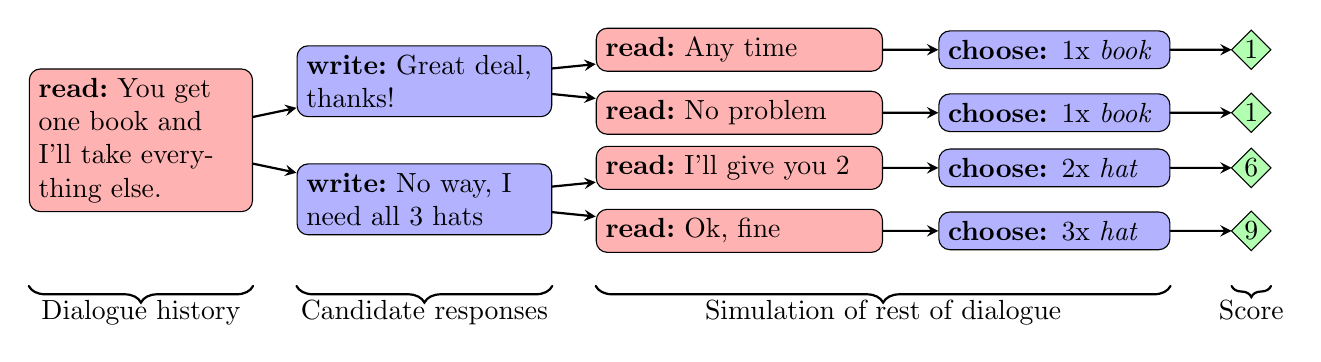
\begin{tikzpicture}[scale=.8,cap=round]
\tikzstyle{them} = [rectangle, rounded corners, minimum width=2cm, text width=2.6cm, minimum height=1cm, draw=black, fill=red!30]
\tikzstyle{candidate} = [rectangle, rounded corners, minimum width=2cm, text width=3cm, minimum height=0.3cm, draw=black, fill=blue!30]
\tikzstyle{rollout} = [rectangle, rounded corners, minimum width=3.4cm, minimum height=0.3cm, text width=3.4cm, draw=black, fill=red!30]
\tikzstyle{score} = [diamond, minimum width=0.5cm, minimum height=0.5cm, draw=black, fill=green!30, inner sep=0,outer sep=0]



\tikzstyle{arrow} = [thick,->,>=stealth]


\node (start) [them] {\them You get one book and I'll take everything else.};
\node (candidate2) [candidate, right of=start, xshift=2.6cm, yshift=0.75cm] {
\you Great deal, thanks!};
\node (candidate1) [candidate, right of=start, xshift=2.6cm, yshift=-0.75cm] {\you No way, I need all 3 hats};
%\node (candidate3) [candidate, below of=candidate2, yshift=-1cm] {Start2};

\node (rollout11) [rollout, right of=candidate1, xshift=3cm, yshift=-0.4cm] {\them Ok, fine};
\node (rollout12) [rollout, right of=candidate1, xshift=3cm, yshift=0.4cm] {\them I'll give you 2};

\node (rollout21) [rollout, right of=candidate2, xshift=3cm, yshift=-0.4cm] {\them No problem};
\node (rollout22) [rollout, right of=candidate2, xshift=3cm, yshift=0.4cm] {\them Any time};


\node (choose11) [candidate, right of=rollout11, xshift=3cm, text width=2.7cm] {\textbf{choose:} 3x \textit{hat}};
\node (choose12) [candidate, right of=rollout12, xshift=3cm, text width=2.7cm] {\textbf{choose:} 2x \textit{hat}};

\node (choose21) [candidate, right of=rollout21, xshift=3cm, text width=2.7cm] {\textbf{choose:} 1x \textit{book}};
\node (choose22) [candidate, right of=rollout22, xshift=3cm, text width=2.7cm] {\textbf{choose:} 1x \textit{book}};


\node (score11) [score, right of=choose11, xshift=1.5cm] {9};
\node (score12) [score, right of=choose12, xshift=1.5cm] {6};

\node (score21) [score, right of=choose21, xshift=1.5cm] {1};
\node (score22) [score, right of=choose22, xshift=1.5cm] {1};



\draw [arrow] (start) -- (candidate1);
\draw [arrow] (start) -- (candidate2);


\foreach \i in {1,2}
{
\draw [arrow] (candidate1) -- (rollout1\i);
\draw [arrow] (candidate2) -- (rollout2\i);

\foreach \j in {1,2}
{
\draw [arrow] (rollout\i\j) -- (choose\i\j);
\draw [arrow] (choose\i\j) -- (score\i\j);
}
}

\draw [
    thick,
    decoration={
        brace,
        mirror,
        raise=1.85cm,amplitude=6pt
    },
    decorate
] (start.west) -- (start.east) node [pos=0.5,anchor=north,yshift=-1.9cm] {Dialogue history}; 

\draw [
    thick,
    decoration={
        brace,
        mirror,
        raise=1.10cm,amplitude=6pt
    },
    decorate
] (candidate1.west) -- (candidate1.east) node [pos=0.5,anchor=north,yshift=-1.15cm] {Candidate responses}; 

\draw [
    thick,
    decoration={
        brace,
        mirror,
        raise=1.5cm,amplitude=6pt
    },
    decorate
] (rollout12.west) -- (choose12.east) node [pos=0.5,anchor=north,yshift=-1.55cm] {Simulation of rest of dialogue}; 

\draw [
    thick,
    decoration={
        brace,
        mirror,
        raise=1.5cm,amplitude=4pt
    },
    decorate
] (score12.west) -- (score12.east) node [pos=0.5,anchor=north,yshift=-1.55cm] {Score}; 


\end{tikzpicture}
\caption{
\label{figure:rollouts} 
对话推演
}\vspace{-2.5mm}
\end{figure*}
与强化学习不同,FAIR在本节利用代理行为概率$p_\theta$计算期望谈判分数,并且这里的计算考虑代理的未来行为,
如图\ref{figure:rollouts}。
FAIR通过两个阶段来实现对话推演。首先,以$U=u_{0..c}$表示整个谈判过程中的表述\wordnote{
    utterances,包括已出现和可能出现的表述。
},以$x_{0..n-1}$表示当前的对话历史。
通过计算$x_{n+k+1,T}$对应的$p_\theta$来获取$u=x_{n,n+k}$。
再通过计算$u=x_{n,n+k}$对应的$R(u)$来挑选最优的输出选择$\vec{o}$。
因此该方法下的期望价值分数与对话中的表述相关:
\begin{equation}
R(x_{n.. n+k})=\mathbb{E}_{x_{(n+k+1.. T;\vec{o})}\sim p_\theta}[r(\vec{o})p_\theta(\vec{o}|x_{0..T})]
\end{equation}

接下来返回最大期望价值分数对应的表述:
\begin{equation}
u^{*}=\argmax_{u\in U}R(u)
\end{equation}

FAIR的对话推演为5次,预测轮数为10轮。
    % \section{实验}
\label{section:experments}
\zihao{-4}

\subsection{Training Details}
FAIR在实验中使用的科学计算工具为PyTorch。
输入的项目数量和价值被嵌入至64维的线性空间,对话中的词则被嵌入至256维的线性空间\wordnote{
    具体的词嵌入方法请参考小节\ref{subsection:grus_rnn}和\citet{  Cho-18,  Cho-28}。
}。
对应的$\text{GRU}_w$,$\text{GRU}_g$,$\text{GRU}_{\overrightarrow{o}}$和$\text{GRU}_{\overleftarrow{o}}$
的隐藏层单元分别为64、128、256和256。

在小节\ref{subsection:supervised_learning}Supervised Learning中,
使用了随机梯度下降的方法搜索预测损失的最小值,其中最小批次采样单元为16个,以此避免落入局域陷阱,
公式\ref{eq:supervised}中的$\alpha$为0.5。
模型的初始学习速度为1.0,Nesterov动量为0.1,梯度速度为0.5。
在此基础训练了30次后,然挑选效果最后的模型结果,并开始对学习速度进行退火处理。

此外,训练与测试数据集中并没有包含人-人谈判失败的情况,且出现次数少于20次的词作废词处理。

在节\ref{section:reinforcement}强化学习中,学习速度为0.1,梯度速度为1.0,公式\ref{eq:reinforcement}中的$\gamma$为0.95。
在4次强化学习后,FAIR同样采用随机梯度下降进行优化,学习速度为0.5。

\subsection{Comparison Systems}
FAIR进行了以下模型谈判比较:
LIKELIHOOD使用了节\ref{section:likelihood}中的supervised training和decoding;
RL使用了节\ref{section:reinforcement}中的goal-based selfplay;
ROLLOUTS使用了节\ref{section:likelihood}中的supervised training和节\ref{section:rollout}中的goal-based decoding;
RL+ROLLOUTS使用了节\ref{section:rollout}中的rollout。

\subsection{Evaluation}
\begin{table*}
\centering
\scalebox{0.85}{\begin{tabular}{c|cccc|cccc|}
\cline{2-9} & \multicolumn{4}{c|}{vs. \likelihood} & \multicolumn{4}{c|}{vs. Human} \\ 
\hline
\multicolumn{1}{|c|}{Model} & \begin{tabular}[c]{@{}c@{}}Score \\ (all)\end{tabular} & \begin{tabular}[c]{@{}c@{}}Score \\ (agreed)\end{tabular}& \begin{tabular}[c]{@{}c@{}}\% \\ Agreed\end{tabular} & \begin{tabular}[c]{@{}c@{}}\% Pareto \\ Optimal\end{tabular} & \begin{tabular}[c]{@{}c@{}}Score \\ (all)\end{tabular} & \begin{tabular}[c]{@{}c@{}}Score \\ (agreed)\end{tabular} & \begin{tabular}[c]{@{}c@{}}\% \\ Agreed\end{tabular}& \begin{tabular}[c]{@{}c@{}}\% Pareto\\ Optimal\end{tabular} \\
\hline
%\multicolumn{1}{l|}{Human} & \multicolumn{1}{l}{} & \multicolumn{1}{l}{} & \multicolumn{1}{l|}{} & \multicolumn{1}{l}{} & \multicolumn{1}{l}{} & \multicolumn{1}{l|}{} \\
\multicolumn{1}{|c|}{\likelihood} & \multicolumn{1}{c}{5.4 vs. 5.5} & \multicolumn{1}{c}{6.2 vs. 6.2} & 
\multicolumn{1}{c}{87.9}& \multicolumn{1}{c|}{49.6} & \multicolumn{1}{c}{4.7 vs. 5.8} & 
\multicolumn{1}{c}{6.2 vs. 7.6} & 
\multicolumn{1}{c}{\textbf{76.5}} &
\multicolumn{1}{c|}{66.2} \\

\multicolumn{1}{|c|}{\reinforce} & \multicolumn{1}{c}{7.1 vs. 4.2} & \multicolumn{1}{c}{7.9 vs. 4.7} & \multicolumn{1}{c}{89.9}& \multicolumn{1}{c|}{58.6} & \multicolumn{1}{c}{4.3 vs. 5.0} & \multicolumn{1}{c}{6.4 vs. 7.5} & \multicolumn{1}{c}{67.3} &\multicolumn{1}{c|}{69.1} \\

\multicolumn{1}{|c|}{\rollouts} & \multicolumn{1}{c}{7.3 vs. 5.1} & \multicolumn{1}{c}{7.9 vs. 5.5} & \multicolumn{1}{c}{92.9}& \multicolumn{1}{c|}{63.7} & \multicolumn{1}{c}{\textbf{5.2 vs. 5.4}} & \multicolumn{1}{c}{7.1 vs. 7.4} & \multicolumn{1}{c}{72.1} &\multicolumn{1}{c|}{78.3} \\

\multicolumn{1}{|c|}{\rlrollouts}  & \multicolumn{1}{l}{\textbf{8.3 vs. 4.2}} & \multicolumn{1}{c}{\textbf{8.8 vs. 4.5}} & \multicolumn{1}{c}{\textbf{94.4}} & \multicolumn{1}{c|}{\textbf{74.8}} & \multicolumn{1}{c}{4.6 vs. 4.2} & \multicolumn{1}{c}{\textbf{8.0 vs. 7.1}} &\multicolumn{1}{c}{57.2} & \multicolumn{1}{c|}{\textbf{82.4}} \\
\hline
\end{tabular}}


\caption{\label{table:endtoend} 模型谈判结果}\vspace{-3.5mm}
\end{table*}
\begin{table}
    \parbox[b]{0.4\textwidth}{
        \centering
        \scalebox{0.80}{\begin{tabular}{|c|c|} 
        \hline
        Metric & Dataset \\ 
        \hline
        Number of Dialogues & 5808  \\
        Average Turns per Dialogue  &  6.6 \\
        Average Words per Turn      &  7.6 \\
        \% Agreed           & 80.1 \\
        Average Score (/10) &  6.0 \\
        \% Pareto Optimal   & 76.9 \\
        \hline
        %Number of words occurring \textgreater10x &         
        \end{tabular}}
        \caption{\label{tab:data} 人-人谈判数据集信息}
        }
    \parbox[b]{0.6\textwidth}{
        \centering
        \scalebox{0.80}{\begin{tabular}{|c|c|c|c|} 
        \hline
        Model & Valid PPL & Test PPL & Test Avg. Rank \\
        \hline
        \likelihood & 5.62 & 5.47 & 521.8 \\
        \reinforce &  6.03 & 5.86   &  517.6  \\
        \rollouts  & - & -   & 844.1 \\
        \rlrollouts & - & - & 859.8 \\
        \hline
        \end{tabular}}
        \caption{\label{table:intrinsic} 词汇复杂度和平均谈判轮数排名}
        }
\end{table}

表\ref{table:endtoend}展示了4种模型分别LIKELIHOOD模型及人类谈判的结果。
评价指标有4种,分别为平均总体得分、平均成交得分、成交率和帕累托最优率。
其中,若两位代理的最终选择出现分歧,即选择的各项目之和不等于初始各项目之和,则视为谈判失败,
所以得分\quotes{Score}分为平均总体得分和平均成交得分;
成交率为谈判成功的次数与总谈判次数的比值;
帕累托最优率为两位代理的输出均已达到价值分数最高,
其中任何一方均没有办法再进行提交的次数与谈判成功次数的比值。

表\ref{tab:data}展示了人-人谈话数据集的结果。

表\ref{table:intrinsic}展示了各模型与人类的差别,其中Valid PPL、Test PPL和Test Avg. Rank分别代表了
LIKELIHOOD模型产生回答的有效复杂度、测试复杂度和平均谈判轮数,指标越低表示越接近人类。
由表\ref{table:intrinsic}可知,LIKELIHOOD模型最接近人。
值得注意的是,模型间的差异有可能是由于RL、ROLLOUTS和RL+ROLLOUTS更复杂化的谈判策略造成的。

通过表\ref{table:endtoend}可知,ROLLOUTS和RL+ROLLOUTS,尤其是RL+ROLLOUTS与LIKELIHOOD模型相比具有明显优势。
RL+ROLLOUTS模型帕累托最优率的提高展示了更好的选择方案,这种结果验证了强化学习与对话推演比单纯模仿人类在谈判上更具有优势。

    % \section{现象}
\label{section:analysis}
\zihao{-4}

\newcommand{\itemvalue}[3]{#2x\textbf{#1} \textit{value}=#3}
\newcommand{\deal[3]}

\begin{table}[t]
    \centering
        \begin{tabular}{|llc|}
        \hline
        \textbf{Input} &&\\
        \rlrollouts{} & \multicolumn{2}{l|}{\itemvalue{book}{4}{0}  \itemvalue{hat}{2}{5}  \itemvalue{ball}{1}{0}}  \\
        Human& \multicolumn{2}{l|}{\itemvalue{book}{4}{1}  \itemvalue{hat}{2}{2}  \itemvalue{ball}{1}{2} }\\
        \hline
        \rlrollouts{}{}    &  \multicolumn{2}{l|}{You can have the ball if I can have everything else.} \\
        Human &  \multicolumn{2}{l|}{No can't do that the ball is not going to give me anything}\\ 
        \rlrollouts{}    &  \multicolumn{2}{l|}{I need the hats and you can have the rest} \\
        Human & \multicolumn{2}{l|}{ Deal} \\ 
        \rlrollouts{}{}    &  \multicolumn{2}{l|}{Great! Thank you!} \\
        \hline
        \textbf{Output} & & \textbf{Reward}\\
        \rlrollouts{} & 2x\textbf{hat} & 10/10\\
        Human &  4x\textbf{book} 1x\textbf{ball} & 6/10 \\
        \hline
        \end{tabular}
\caption{\label{table:example}模型示例}
\end{table}

RL+ROLLOUTS模型的谈判明显要比LIKELIHOOD模型花费更多的轮数,这表明RL+ROLLOUTS谈判起来更加努力。
但在一些情景下,RL+ROLLOUTS模型更倾向在每一轮中坚持价值最大的需求仅做出表述方式上的改变。
这在实际与人类谈判时,人类更有可能在较少轮数内直接放弃谈判而不会像机器一样接受或是最终disagree。

欺骗是一种高级的谈判策略,FAIR发现RL+ROLLOUTS模型在某些情景中假装对价值底的项目感兴趣,最终\quotes{妥协}
取得高价值项目,
如表\ref{table:example}。

FAIR认为此篇论文所提出的模型能够产生流畅的对话语句。
不过个人通过观察数据集认为,首先训练集和测试集中的人-人对话语句内词汇量较少,语法结构较为简单。
因此流畅的对话语句不足为奇。FAIR也提出会在将来扩充表述的多样性。

FAIR发现RL+ROLLOUTS模型的一种语言错误普遍发生在agreement的语境下却提出了更进一步的要求即counter offer。
这一行为很少在人类身上发生。
FAIR认为出现这种情况的原因在于,在训练集中,agree往往处于谈判结束前,而且对方代理很少就agree再进行谈判。
因此,RL+ROLLOUTS模型可能认为在谈判快要提出agree时进行counter offer有助于对方接收该要求。

    % \nocite{*}
    \bibliography{_citation}
    % \nocite{*}
    \bibliographystyle{unsrtnat}
\end{document}